% Options for packages loaded elsewhere
\PassOptionsToPackage{unicode}{hyperref}
\PassOptionsToPackage{hyphens}{url}
%
\documentclass[
  a4paper,
]{article}
\usepackage{amsmath,amssymb}
\usepackage{lmodern}
\usepackage{ifxetex,ifluatex}
\ifnum 0\ifxetex 1\fi\ifluatex 1\fi=0 % if pdftex
  \usepackage[T1]{fontenc}
  \usepackage[utf8]{inputenc}
  \usepackage{textcomp} % provide euro and other symbols
\else % if luatex or xetex
  \usepackage{unicode-math}
  \defaultfontfeatures{Scale=MatchLowercase}
  \defaultfontfeatures[\rmfamily]{Ligatures=TeX,Scale=1}
\fi
% Use upquote if available, for straight quotes in verbatim environments
\IfFileExists{upquote.sty}{\usepackage{upquote}}{}
\IfFileExists{microtype.sty}{% use microtype if available
  \usepackage[]{microtype}
  \UseMicrotypeSet[protrusion]{basicmath} % disable protrusion for tt fonts
}{}
\makeatletter
\@ifundefined{KOMAClassName}{% if non-KOMA class
  \IfFileExists{parskip.sty}{%
    \usepackage{parskip}
  }{% else
    \setlength{\parindent}{0pt}
    \setlength{\parskip}{6pt plus 2pt minus 1pt}}
}{% if KOMA class
  \KOMAoptions{parskip=half}}
\makeatother
\usepackage{xcolor}
\IfFileExists{xurl.sty}{\usepackage{xurl}}{} % add URL line breaks if available
\IfFileExists{bookmark.sty}{\usepackage{bookmark}}{\usepackage{hyperref}}
\hypersetup{
  pdftitle={Sensorimotor Learning of a Virtual Skill},
  pdfauthor={Spencer R. Wilson},
  hidelinks,
  pdfcreator={LaTeX via pandoc}}
\urlstyle{same} % disable monospaced font for URLs
\usepackage[margin=30mm]{geometry}
\usepackage{graphicx}
\makeatletter
\def\maxwidth{\ifdim\Gin@nat@width>\linewidth\linewidth\else\Gin@nat@width\fi}
\def\maxheight{\ifdim\Gin@nat@height>\textheight\textheight\else\Gin@nat@height\fi}
\makeatother
% Scale images if necessary, so that they will not overflow the page
% margins by default, and it is still possible to overwrite the defaults
% using explicit options in \includegraphics[width, height, ...]{}
\setkeys{Gin}{width=\maxwidth,height=\maxheight,keepaspectratio}
% Set default figure placement to htbp
\makeatletter
\def\fps@figure{htbp}
\makeatother
\setlength{\emergencystretch}{3em} % prevent overfull lines
\providecommand{\tightlist}{%
  \setlength{\itemsep}{0pt}\setlength{\parskip}{0pt}}
\setcounter{secnumdepth}{5}

%% pandoc-fignos: required package
\usepackage[capitalise]{cleveref}
\ifluatex
  \usepackage{selnolig}  % disable illegal ligatures
\fi
\newlength{\cslhangindent}
\setlength{\cslhangindent}{1.5em}
\newlength{\csllabelwidth}
\setlength{\csllabelwidth}{3em}
\newenvironment{CSLReferences}[2] % #1 hanging-ident, #2 entry spacing
 {% don't indent paragraphs
  \setlength{\parindent}{0pt}
  % turn on hanging indent if param 1 is 1
  \ifodd #1 \everypar{\setlength{\hangindent}{\cslhangindent}}\ignorespaces\fi
  % set entry spacing
  \ifnum #2 > 0
  \setlength{\parskip}{#2\baselineskip}
  \fi
 }%
 {}
\usepackage{calc}
\newcommand{\CSLBlock}[1]{#1\hfill\break}
\newcommand{\CSLLeftMargin}[1]{\parbox[t]{\csllabelwidth}{#1}}
\newcommand{\CSLRightInline}[1]{\parbox[t]{\linewidth - \csllabelwidth}{#1}\break}
\newcommand{\CSLIndent}[1]{\hspace{\cslhangindent}#1}

\title{Sensorimotor Learning of a Virtual Skill}
\author{Spencer R. Wilson}
\date{\today}

\usepackage[capitalise]{cleveref}
\usepackage{graphicx}
\graphicspath{{/Users/spencerw/Google Drive/motor_control/phd/}}
\usepackage{subfigure}

\begin{document}
\maketitle

\hypertarget{sec:intro}{%
\section{Introduction \& Aims}\label{sec:intro}}

\begin{quote}
\emph{Movement is nothing but the quality of our being.}

--- Sunryu Suzuki, \emph{Zen Mind, Beginner's Mind}
\end{quote}

The purpose of this thesis is to construct a high-dimensional
electromyography recording setup as a platform on which a suite of motor
control and learning experiments can be explored. With this novel setup,
we hope to advance our understanding of trial-to-trial motor learning
through the combination of experiment and theory.

A recent review provides a clear call to action for work this direction:

\begin{quote}
The processes by which biological control solutions spanning large and
continuous state spaces are constructed remain relatively unexplored.
Future investigations may need to embed rich dynamical interactions
between object dynamics and task goals in novel and complex
movements.\textsuperscript{\protect\hyperlink{ref-McNamee2019}{1}}
\end{quote}

Over the last few decades, there has been considerable amount of work
done to untangle the abilities of the motor system to flexibly control
the body including through optimal control
theory\textsuperscript{\protect\hyperlink{ref-Todorov2004}{2}},
reinforcement learning in continuous action
space\textsuperscript{\protect\hyperlink{ref-koberReinforcementLearningRobotics2013}{3}},
and detailed physiological
studies\textsuperscript{\protect\hyperlink{ref-sauerbreiCorticalPatternGeneration2019}{4}}.
However, as the quote above suggests, a holistic understanding of the
computations underlying the construction of skilled movement remains an
exciting direction for research. Our aim is to progress understanding of
skilled movement by studying the solutions produced by human subjects to
motor tasks in dynamically rich, yet controlled, virtual environments.
Our goal is to reverse-engineer the ability to acquire and perform novel
motor skills.

Humans produce a great variety of movements every day, often without
conscious thought. For example, movements like bringing a cup of coffee
to our lips for a sip are generally out of reach for state-of-the-art
robotic systems. We claim that this ``motor gap'' between biological and
artificial motor systems is due to a lack of \emph{dexterity}. Soviet
neuroscientist Nikolai Bernstein defined dexterity as the ability to
``find a motor solution in any situation and in any
condition.''\textsuperscript{\protect\hyperlink{ref-Bernstein1967}{5}}
The crux of this definition is the flexibility of such solutions. This
flexibility, or
robustness\footnote{Kitano defines robustness as ``the maintenance of
  specific functionalities of the system against perturbations, and it
  often requires the system to change its mode of operation in a
  flexible way.'' He claims that robustness requires control,
  alternative mechanisms, modularity and decoupling between high and low
  level variability.}\textsuperscript{\protect\hyperlink{ref-kitanoBiologicalRobustness2004}{6}},
is the ability to optimize internal parameters in response to external
perturbations and adapt to new information to achieve the goals of an
ongoing plan.

To explore dexterous movement, we will leverage recordings of muscles
controlling the hand as a readout of flexible motor behavior. This is a
step beyond recording hand kinematics as electromyography provides a
physiological output of the nervous system. Surface electromyography
recordings taken from the forearms controlling subjects' dominant hands
allows us to track the sequential selection of muscle activations during
both skill acquisition and subsequent performance of that skill to
achieve desired goal. As we are interested in subjects' abilities to
acquire new skills, we design tasks that require subjects to use
available, but uncommon, motor activations. We then track the selection
and execution of these activation during virtual tasks. Preliminary work
in this direction is described in \cref{sec:experiment}.

Using data from our experimental setup, we wish to understand both how
the structure of muscle activation variability evolves during skill
acquisition and how the motor system constructs skilled movement through
the composition of component muscle activations. To begin, we review a
sampling of current motor physiology research relevant to dexterous
motor computations in \cref{sec:physiology}. In \cref{sec:experiment},
we cover our prototype hardware and experiments. With inspiration from
physiology and our experiments, we hope to make progress in modeling
sensorimotor control and learning in our experimental setup. We cover
preliminary work in this direction in \cref{sec:theory}, and discuss
possible future directions in \cref{sec:next_steps}.

\clearpage

\hypertarget{sec:physiology}{%
\section{Reverse Engineering the Movement
Machine}\label{sec:physiology}}

\begin{quote}
\emph{Even a simple movement is a global body event.}

--- Bizzi \& Ajemian, \emph{2020}
\end{quote}

\hypertarget{motor-units-to-muscles}{%
\subsection{Motor Units to Muscles}\label{motor-units-to-muscles}}

The quantum of motor output is the motor unit (MU), defined as a single
motoneuron axon and the set of junctions the terminals of its axon
branches form with one or more muscle fibers. The MU provides the motor
system with spatial redundancy at the muscle level: multiple muscle
fibers contract due to a single alpha motoneuron (AMN) spike in the
spinal cord's ventral horn, and multiple AMNs may overlap in their
innervations. The forces produced by motor units span several orders of
magnitude, though most units produce very small forces. Here we find
temporal redundancy: in order to produce movements, MUs combine to
generate a range of
forces\textsuperscript{\protect\hyperlink{ref-fuglevandMechanicalPropertiesNeural2011}{7}}.
Since the innervation ratios of muscles in the forearm and hand are
relatively small compared to more proximal muscles (which contain
thousands of MUs), the logarithmic recruitment and redundancy of motor
units enables the hand to produce movements with very fine
spatiotemporal resolution.

Muscle fibers are contained within muscle compartments, and each muscle
may have one or more compartments. The fingers of the hand are extended
by the extensor digitorum (ED) which contains four compartments, one for
each of the tendons the muscle produces. Each tendon connects to the
three metaphalangeal joints of each digit. The fingers are flexed by two
muscles, the flexor digitorum superficialis (FDS) and the flexor
digitorum profundus (FDP). Like the ED, these muscles produce four
tendons, one to each finger from each of their four compartments. As
such, one must coactivate these agonist and antagonist muscles in order
to extend or flex a single finger in
isolation\textsuperscript{\protect\hyperlink{ref-fuglevandMechanicalPropertiesNeural2011}{7}}.
Adduction and abduction of the fingers is produced by the 19 intrinsic
muscles of the hand, each of which has their origin and insertion points
within the hand
itself\textsuperscript{\protect\hyperlink{ref-vanduinenConstraintsControlHuman2011}{8}}.
The intrinsic muscle tendons form a kind of network around each of the
digits. The human hand, thumb, and forearm system contains more than 30
muscles and at least 20 degrees of freedom are theoretically available
for actuation. However, due to biomechanical coupling, the effective
degrees of freedom is presumably less than 20.

This structure exists in order to facilitate the acquisition of new
skills and the generalization of existing skills to new contexts. While
the anatomy of the hand and forearm presents constraints on movement,
the system remains capable of producing an incredible variety of
movement
patterns\textsuperscript{\protect\hyperlink{ref-yanUnexpectedComplexityEveryday2020}{9},\protect\hyperlink{ref-Basmajian1963}{10}}\footnote{In
  a classic study, Basmajian and colleagues showed that it is possible
  to activate single motor units in the thumb abductor.}. The structure
of the neuromuscular system that underlies this variety offers many
clues as to the relevant computations required for dexterous movement.
In \cref{fig:low_variance_PCs}, Yan et al.~show how even low-variance
principle components of joint kinematics during object grasping and ASL
signing display correlational structure and not merely noise. That is,
the production of hand movement is highly task-specific, where
individual tasks are linked to bespoke muscle activations patterns.

\begin{figure}
\hypertarget{fig:low_variance_PCs}{%
\centering
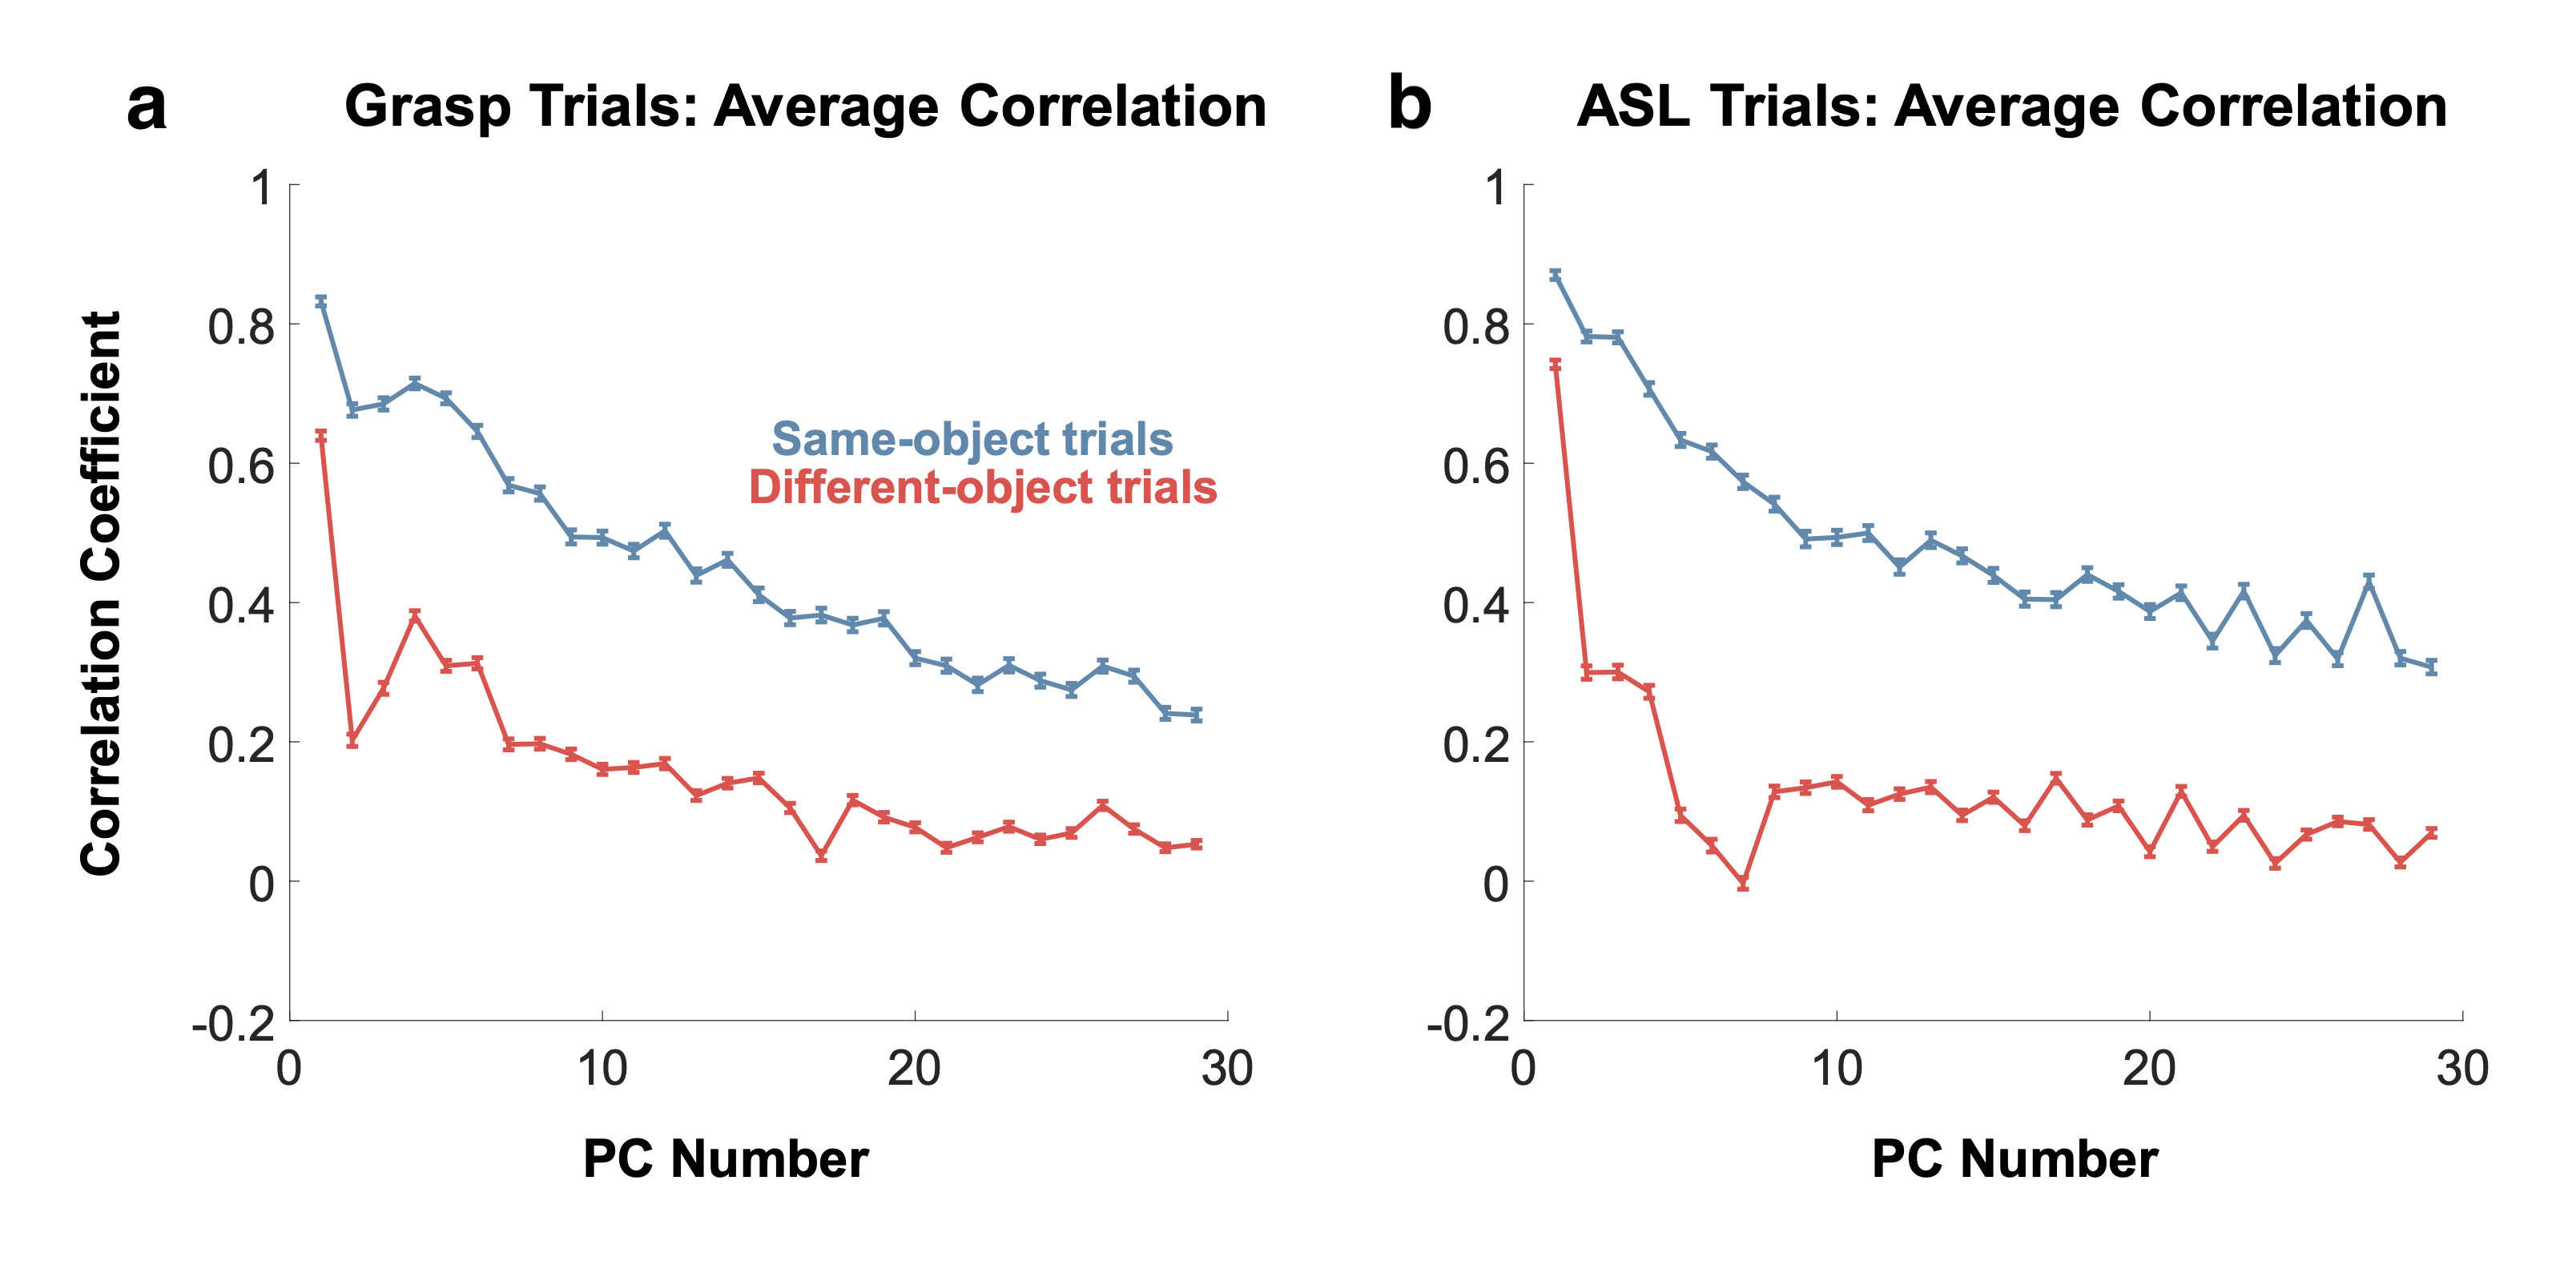
\includegraphics[width=1\textwidth,height=\textheight]{images/physiology/background/low_variance_PCs.png}
\caption{Taken from Yan et al.~2020. Plots show mean correlations
between hand joint kinematic trajectories during grasp trials with the
same (blue) and different (red) objects (a) and ASL signs (b) projected
onto the same principle components. Correlations are averaged across 8
subjects. Within-object and within-sign correlations are systematically
higher than their shuffled counterparts. Error bars denote SEM. This
data supports the idea that low-variance components of kinematics data
contain task-specific structure rather than merely reflecting noise.
This is encouraging for our experiments, which hope to extend this idea
into careful analyses of task specific features of EMG data across
learning and in response to perturbations.}\label{fig:low_variance_PCs}
}
\end{figure}

\hypertarget{coordinative-structures}{%
\subsection{Coordinative Structures}\label{coordinative-structures}}

Many studies have contributed to the concept of synergies as a
hard-wired organizing feature of the motor
system\textsuperscript{\protect\hyperlink{ref-DAvella2003}{11}}.
However, these works tend to extrapolate from non-primate preparations,
particularly in the frog, and use tasks which are inherently
low-dimensional to explain covariance structure in primate and human
kinematic and electromyography
data\textsuperscript{\protect\hyperlink{ref-giszterMotorPrimitivesNew2015}{12},\protect\hyperlink{ref-gao2017}{13}}.
That said, it would be foolish to deny the existence of synergistic
muscle coactivation even at the structural level. Careful studies of
force control by the fingertips present a complex story of
dimensionality of control in this
regime\textsuperscript{\protect\hyperlink{ref-raczSpatiotemporalAnalysisReveals2013}{14}}.
Constraints exist in the architecture of the hand as well as its control
system, though we maintain that concept of synergies, especially in the
context of dexterous movement, is often presented as an
oversimplification rather than a mere simplification. We believe the
story of the hand is more complex.

Studies have attempted to quantify the number of effective degrees of
freedom of the hand with various methods. This has primarily been taken
to be the number of linear features which contain a desired level of the
original signal variance, where the signal is the joint angles of the
hand engaged in various
behaviors\textsuperscript{\protect\hyperlink{ref-Ingram2009}{15},\protect\hyperlink{ref-TodorovDimensionality2005}{16}}.
These methods have resulted in roughly 8 linear features of hand
kinematics to solve a variety of tasks, with subtleties found in
inter-task and inter-subject variations. Note that the motor repertoire
is hardly high-dimensional when compared to the dimensionality of the
visual feature extraction
system\textsuperscript{\protect\hyperlink{ref-yanUnexpectedComplexityEveryday2020}{9}}.
A recent study found that low-variance linear, kinematic components
displayed significantly higher correlation within condition (e.g.~grasp
of a specific object) than across condition. This suggests that these
components carry task-dependent information rather than
condition-independent, task-irrelevant
noise\textsuperscript{\protect\hyperlink{ref-yanUnexpectedComplexityEveryday2020}{9}}.
This suggests that the control of the hand is more nuanced than a set of
fixed synergies.

What Bizzi and colleagues call ``the problem of supraspinal pattern
formation''--how synergies are activated through time-- we argue, in the
context of hand control, is not simplified by the existence of
hard-wired or soft-wired
synergies\textsuperscript{\protect\hyperlink{ref-bizziMotorPlanningExecution2020}{17}}.
Rather, the CNS produces control signals in a range of contexts and in
response to continually changing task demands. Rather than the CNS
``simplifying movement'' through synergetic action, it is more likely
that hand synergies fall out of a optimization strategy which trades off
effort and accuracy where effort may, in part, correspond to independent
control of individual control dimensions. In this view, synergies,
hard-wired or not, reflect the statistics of the environment in which
movement is
constructed\textsuperscript{\protect\hyperlink{ref-brutonSynergiesCoordinationComprehensive2018}{18}}.
If we limit ourselves to synergetic control, then we have simply passed
the problem to a lower-dimensional one of the same fundamental nature.
Neural control of the hand likely contains a spectrum of modularity in
order to maintain its role as a flexible instrument. Synergetic action
is one end of this spectrum resulting from the computations inherent to,
along with the structures of the human movement machine.

\hypertarget{fractionating-structures}{%
\subsection{Fractionating Structures}\label{fractionating-structures}}

Just as many muscle fibers may be innervated by a single AMN, up to
thousands of neurons contact single AMNs through monosynaptic
corticospinal, or corticomotoneuronal (CM), connections and other
descending pathways through elaborate spinal circuitry. The hallmark of
CM connections in particular is their influence over multiple muscle
compartments as well as multiple muscles, though typically agonist or
antagonist
sets\textsuperscript{\protect\hyperlink{ref-cheneyFunctionalClassesPrimate1980}{19}}.
This may seem counter-intuitive as a means to produce individuated
movement, but experimental evidence in primates has shown that the
convergence of many CM collateral fibers onto single AMNs driving the
distal muscles in particular can produce a fine grading of activity over
motor units driving the distal joints. CM cells also appear to play a
role in the inhibition of antagonist muscles prior to contractions
required for
movement.\textsuperscript{\protect\hyperlink{ref-griffinMotorCortexUses2020}{20}}
These findings confirm theories about the excitatory and inhibitory role
of these connections dating back decades, and combine to suggest that
variables encoded in cortical ensembles are more complex than kinematics
or dynamics
alone\textsuperscript{\protect\hyperlink{ref-cheneyFunctionalClassesPrimate1980}{19}}.

The CM tract thus acts in coordination with synergistic muscle
activations of the hand to achieve control that is balanced between
modularity and flexibility. Findings suggest that there is a bipartite
structure in human motor cortex driving dexterous control of the distal
part of the upper limb which, it has been suggested, evolved under
pressure to quickly generalize between tasks. This work argues that
these two streams of hand control, namely ``fractionated'' and
``synergistic'' control, may interact to produce versatility, and
balancing these subsystems may be a key part of the optimization
function when learning new
skills\textsuperscript{\protect\hyperlink{ref-Rathelot2009}{21}--\protect\hyperlink{ref-Takei2017}{23}}.
This dualism is likely not rigidly dichotomous, but rather a spectrum of
overriding fractionation (so-called ``New M1'') atop a phylogenetically
older system of synergistic
action\textsuperscript{\protect\hyperlink{ref-dumCorticospinalSystemStructural2011}{24}}.
Griffin and colleagues found that CM cells are functionally tuned to a
muscle's mode of activity (agonist, antagonist, fixator) to ``bypass
spinal cord mechanisms and sculpt novel patterns of motor output that
are essential for highly skilled
movements''\textsuperscript{\protect\hyperlink{ref-griffinCorticomotoneuronalCellsAre2015}{22}}.
The hypothesis stemming from the previously described work is that CM
connections override the ``consolidated'' patterns putatively generated
via spinal interneuron circuitry. The setup devised in our work aims to
measure fractionation by tracing motor unit correlations across
learning. Whether fractionation in our experiments is due to the CM
pathway can only be speculation, but our work may provide direction for
future studies pairing intracortical recordings with careful
electromyography.

\hypertarget{supraspinal-motor-maps}{%
\subsection{Supraspinal Motor Maps}\label{supraspinal-motor-maps}}

It is known from recent work that primary motor cortex (M1) is not an
isolated movement-generating dynamical system, but rather a node in the
network of a feedback-modulated, distributed movement
machine\textsuperscript{\protect\hyperlink{ref-sauerbreiCorticalPatternGeneration2019}{4}}.
Thinking of the structural architecture of M1 as an input-driven system
with outputs along a spectrum of modularity from synergistic to
fractionated, we can ask what kind of functional architecture might have
evolved in the neuromuscular controller? Graziano and colleagues found
that 500ms electrical stimulation to M1 reliably produced stereotyped
movements in
primates\textsuperscript{\protect\hyperlink{ref-graziano2006}{25}}.
These movements appeared to produce goal-oriented actions pulled out of
other contexts such as bringing food to the mouth, and seemed to be
arranged on the cortical sheet topographically in terms of spatial
endpoints rather than as a humunculus. Graziano refers to this as the
cortical ``action map'', that these stimulations tapped into the control
mechanisms of the primate's motor
system\textsuperscript{\protect\hyperlink{ref-grazianoIntelligentMovementMachine2009}{26}}.
These results has recently been confirmed by optogenetics work in
marmosets and
macaques.\textsuperscript{\protect\hyperlink{ref-ebina2019}{27},\protect\hyperlink{ref-watanabeForelimbMovementsEvoked2020}{28}}

The motor map concept suggests interpreting activity in M1 as a field of
feedback control microcircuits, integrating and transforming inputs,
both internal and external, to sculpt ongoing
movement\textsuperscript{\protect\hyperlink{ref-wiltschkoMappingSubSecondStructure2015}{29}}.
This is in accordance with the idea that there is a structural hierarchy
in M1 covering a spectrum of movement modularity. These ideas together
form a picture of the motor system as a structural scaffold upon which
behaviorally relevant feedback mappings from cortex to the spinal cord
are continuously activated and modulated based on information and
estimates about the periphery. In this view, the encoded variables of
interest depend on the goals, context, and perturbations of the intended
movement. \cref{fig:strick_graziano} shows Graziano et al.'s stimulation
results, what might be termed a functional view of the cortical motor
system, next Strick er al.'s described above clarifying the structural
view of modularity in this system.

\begin{figure}
\hypertarget{fig:strick_graziano}{%
\centering
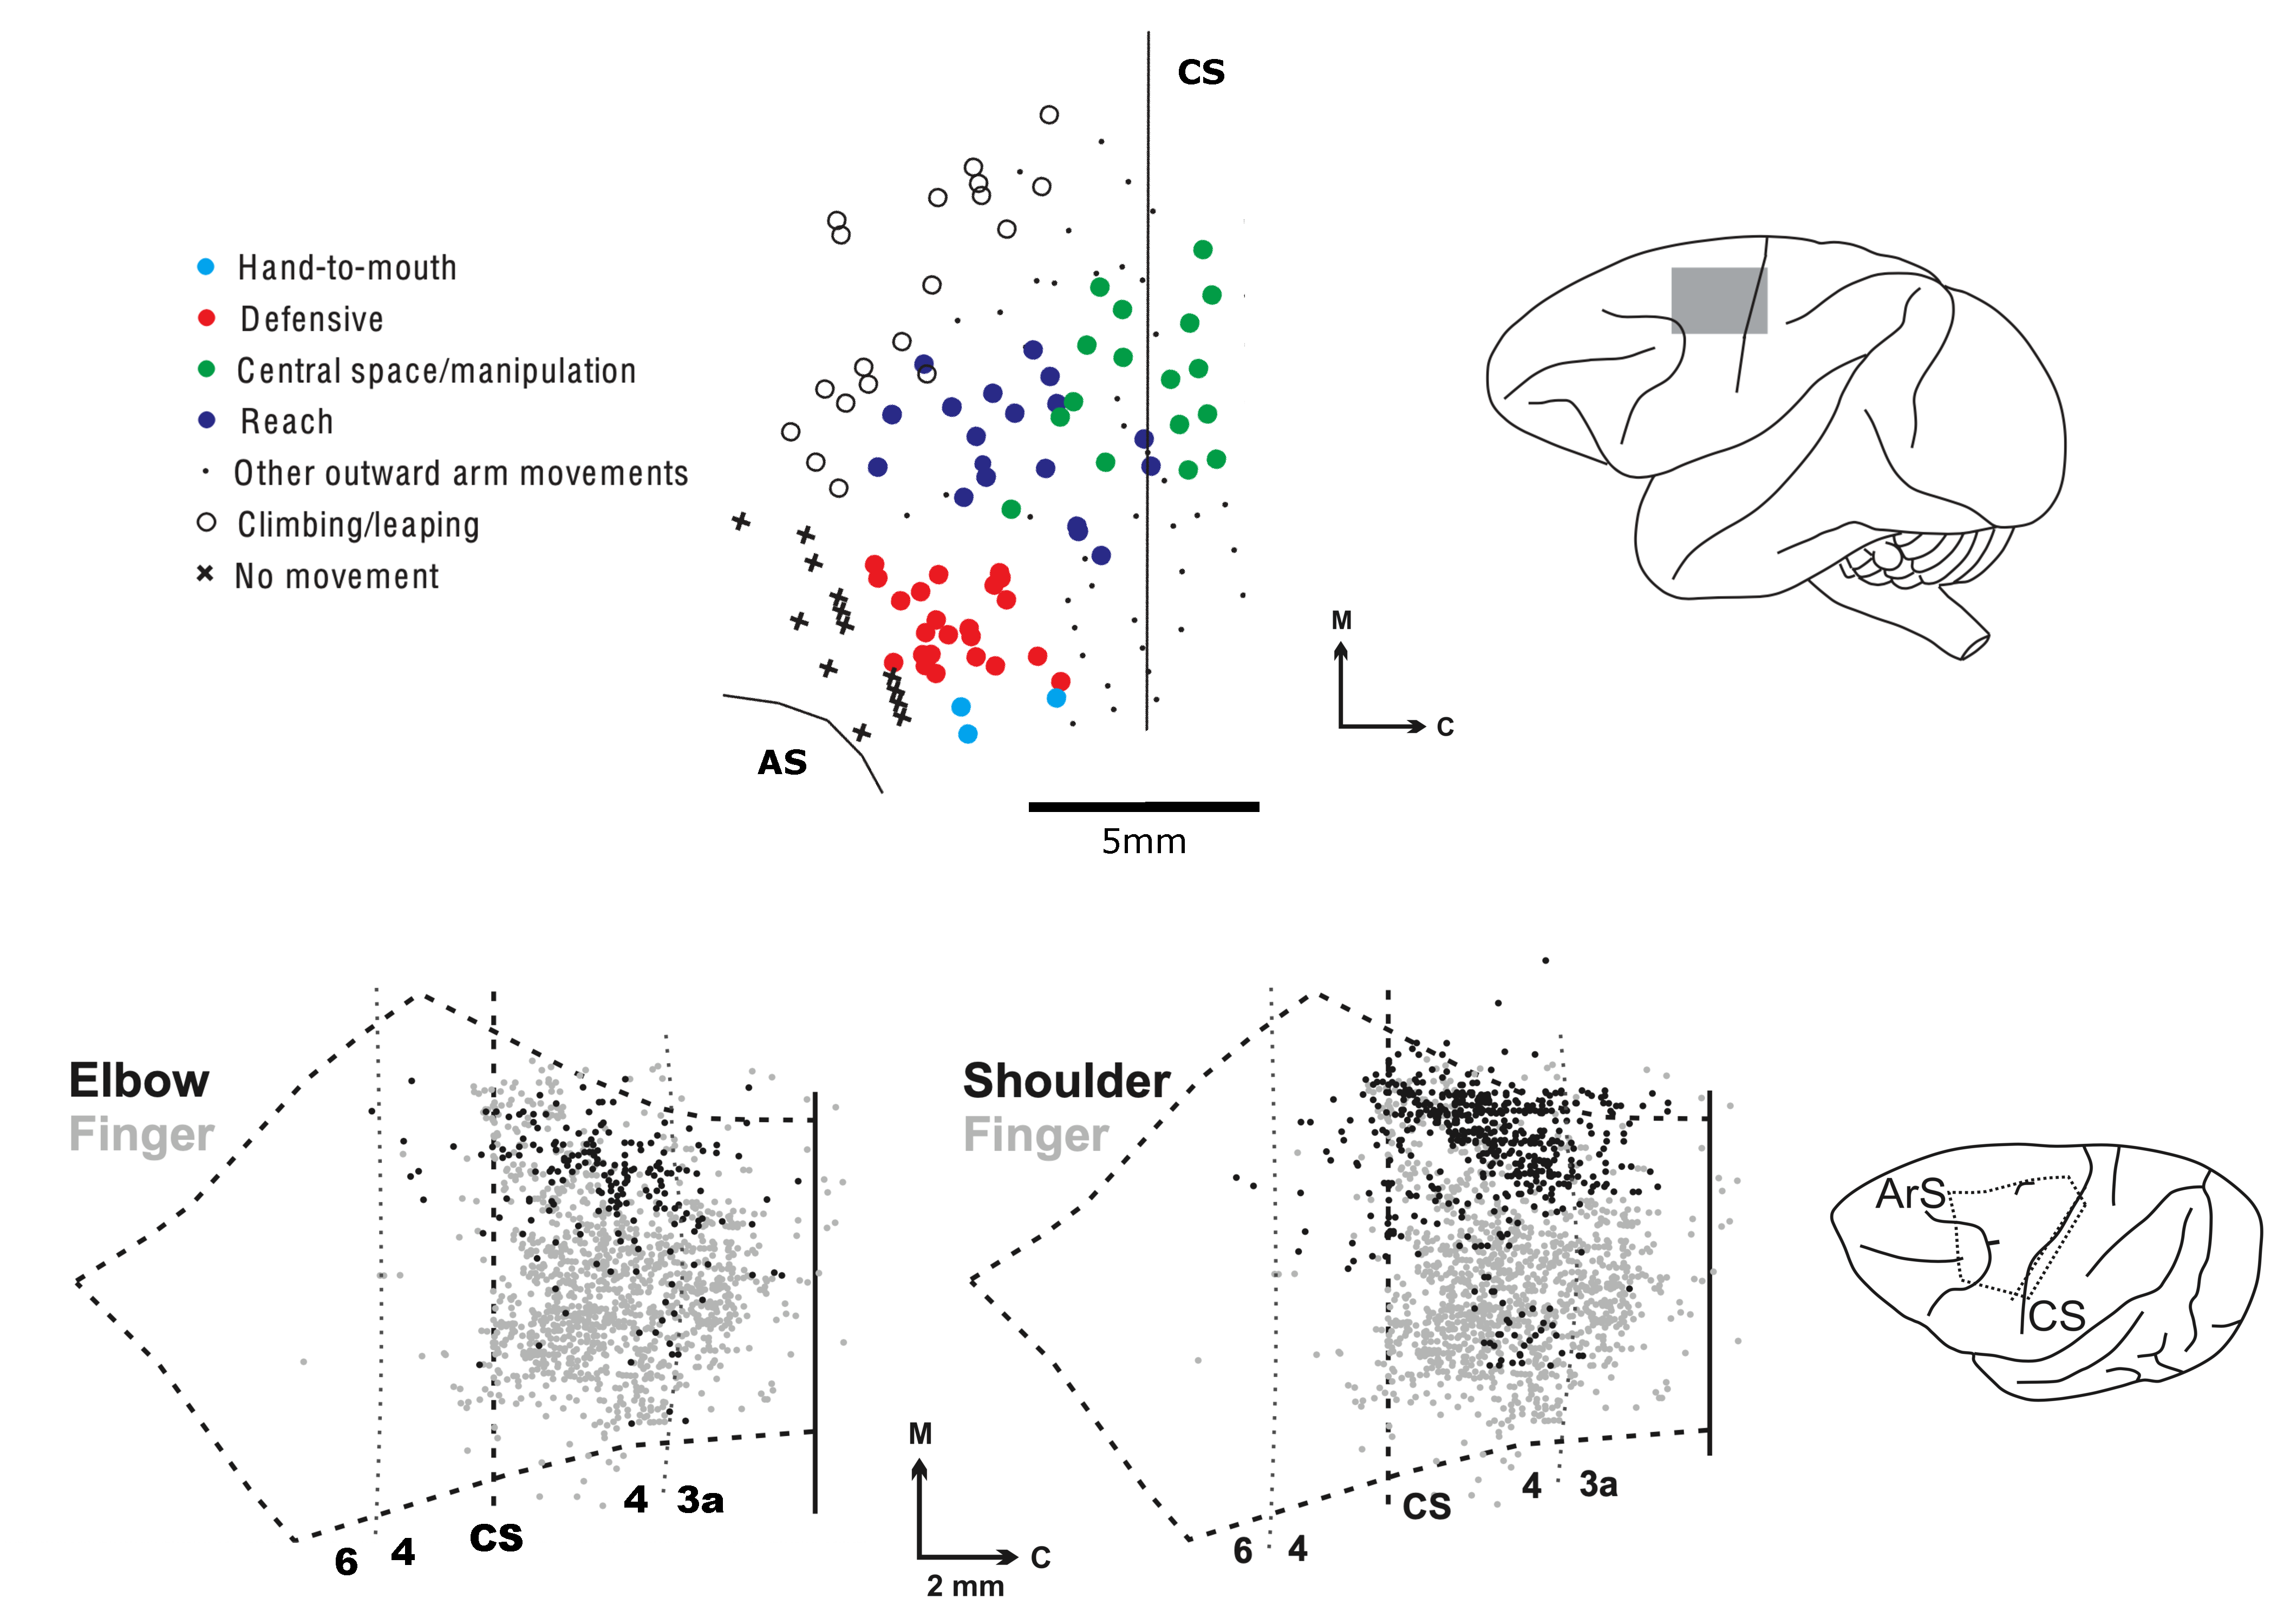
\includegraphics[width=1\textwidth,height=\textheight]{images/physiology/strick_graziano/strick_graziano.pdf}
\caption{Similarities between electrical stimulation on behavorial
timescales and rabies tracing identification of CM cells. CM cells are
largely confined to the caudal half of M1, while this region tends to
evoke complex manipulatory movements when electrically stimulated. (Top
Left) Corticomotoneuronal (CM) cells traced using rabies from muscles of
the elbow and finger. (Top Right) CM cells traced using rabies from
muscles of the shoulder and finger. (Bottom) Complex movements evoked by
500ms electrical stimulation pulse trains. Adapted from Graziano 2005
and Rathelot et
al.~2009\textsuperscript{\protect\hyperlink{ref-Rathelot2009}{21},\protect\hyperlink{ref-graziano2005}{30}}.}\label{fig:strick_graziano}
}
\end{figure}

Graziano writes:

\begin{quote}
``The usefulness of a feedback-dependent mapping from cortex to muscles
is that it can in principle allow neurons in motor cortex to control a
diversity of movement variables, such as direction, speed, hand
position, or posture that transcend a fixed pattern of muscle
activation. If the network receives feedback information about a
specific movement variable, then it can learn to control that
variable.''
\end{quote}

Muscle activity is, in this sense, a readout from a network transforming
state-dependent inputs into movement goals. Rather than choosing muscle
patterns in reconfigurable blocks, it creatively constructs and sculpts
movement. The hierarchy of the motor system may not be rigidly organized
around a particular set of variables. As shown in
\cref{fig:motor_system}, many loops exist connecting cortex with the
spinal cord, the cerebellum, the basal ganglia, and the sensorimotor
periphery. Each of these loops contributes information for the flexible
activation of the relevant action maps. Put simply, prevailing evidence
suggests that cerebellar loops provide predictive state information
while basal gangliar loops provide state and/or action value
information. Taken together, this work provides an image of the
incredible complexity which generates dexterous movements of the hand.
This is the foundation on which we can work to build experiments which
elucidate the computations involved in the production of skilled
movement. We aim to connect our results back to what is known about the
system we are attempting to reverse-engineer in order to inspire future
inquiries into the inner workings of the movement machine.

\begin{figure}
\hypertarget{fig:motor_system}{%
\centering
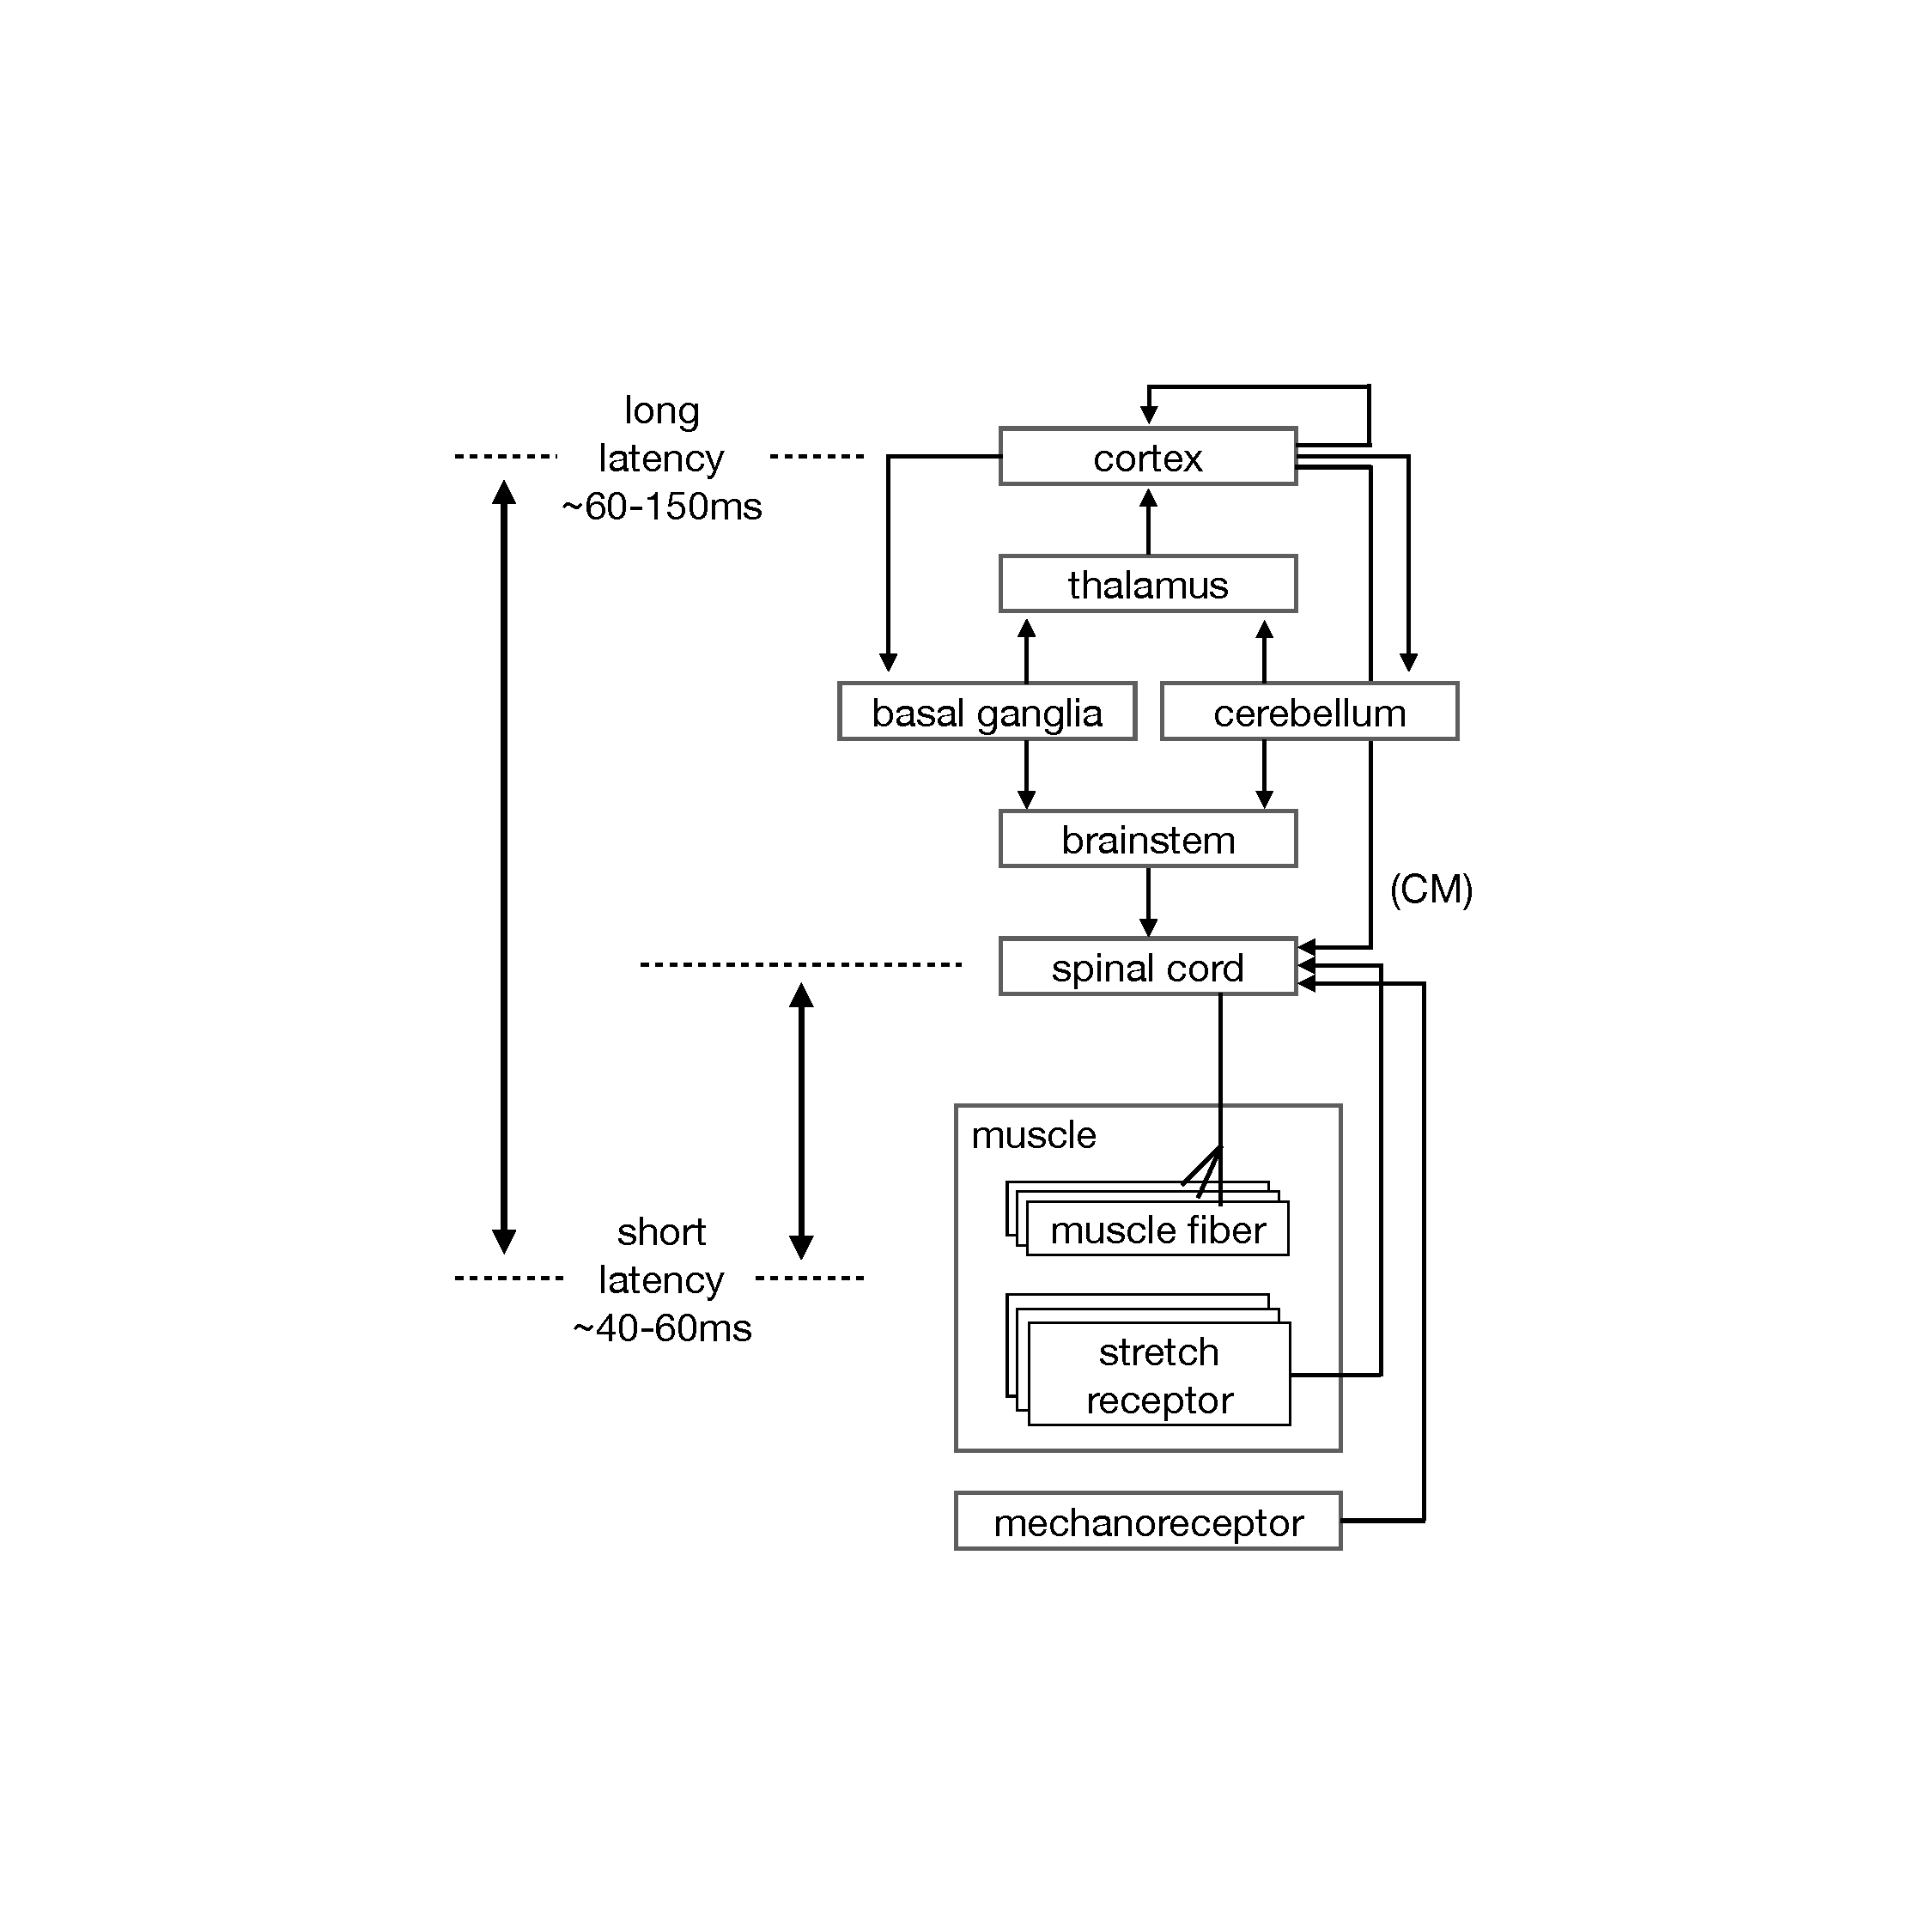
\includegraphics[width=1\textwidth,height=\textheight]{images/physiology/motor_system/motor_system.pdf}
\caption{Overview sketch of the motor system depicting the the
redundancy of the system both hierarchically (multiple muscle fibers are
innervated by the same motor neuron, many motor neurons innervate the
same muscle) as well as heterarchically (parallel spinal,
corticomotoneuronal, cerebellum, basal gangliar feedback loops).
Parallel reflex responses can be classified as long latency
(approximately 60-150ms) and short latency (approximately 60ms). We hope
to consider the parallelism and redundancy of the motor system to
inspire our data analyses and models of motor
computation.}\label{fig:motor_system}
}
\end{figure}

\clearpage

\hypertarget{sec:experiment}{%
\section{Preliminary Experiments}\label{sec:experiment}}

\begin{quote}
\emph{We have some idea as to the intricate design of the puppet and the
puppet strings, but we lack insight into the mind of the puppeteer.}

--- Bizzi \& Ajemian, \emph{2020}
\end{quote}

\hypertarget{recording-setup}{%
\subsection{Recording Setup}\label{recording-setup}}

The concept of the experimental setup is shown in \cref{fig:setup},
where 32 monopolar electrodes are attached to a subject's forearm to
record muscle activity. The arm and hand are kinematically constrained
in a custom fixture and motor activity is recorded during low-level
isometric muscle contractions. The setup circumvents the limb
biomechanics by mapping muscle output directly to virtual stimuli shown
on a screen. By focusing on low-force, isometric contractions we intend
to avoid complications due to artifacts in dynamic, high-force
movements.

\begin{figure}
\hypertarget{fig:setup}{%
\centering
\includegraphics[width=1\textwidth,height=\textheight]{images/hardware/setup.pdf}
\caption{(a) Graphic depicting the closed-loop EMG interface concept in
a center-hold, reach-out type task. The multidimensional EMG signal is
transformed online through a mapping \(F\) from EMG electrode space to a
lower dimensional task space. In experiments shown here the task space
is a two-dimensional, though the EMG interface can be extended to tasks
with higher-dimensional inputs. The subject's arm and hand are
constrained during the experiment to ensure isometric contractions. (b)
First prototype of custom recording hardware consisting of four bands of
eight electrodes each, and a spherical hand constraint. Our recordings
are 32 channel monopolar recording with reference electrode at the
wrist. (c) Example cup-style monopolar recording electrodes, 5mm in
diameter. (d) Side view of the recording hardware. Also pictured is the
arm restraint frame to ensure isometric contractions. The frame obscures
the subject's arm from view and contains adjustable elbow and wrist
rests. (d) Recording hardware shown off the arm with wireless amplifier
and connection board.}\label{fig:setup}
}
\end{figure}

As far as we are aware, this setup is novel in combining a high number
of channels with an abstract mapping. Learning experiments have used
joint angles and a few muscles (typically movements of the wrist or
pairs of thumb and intrinsic hand muscles), but none have taken a
data-driven approach in constructing a virtual learning environment in
the style of cortical
BMI\textsuperscript{\protect\hyperlink{ref-BergerDifferencesInAdaptationRates2013a}{31}--\protect\hyperlink{ref-Gallego2017}{34}}.
Our EMG recording setup is custom-built: the ``Sessantaquattro'' EMG
amplifier was acquired from OT Bioelettronica, the electronic connector
was designed in-house, the electrodes were acquired from Medkit UK, and
the recording software was written in a mixture of Bonsai (C\#) and
Python. EMG is acquired at 2kHz sample rate with 24-bit precision. A
clip of raw data is shown in \cref{fig:raw_data}.

\begin{figure}
\hypertarget{fig:raw_data}{%
\centering
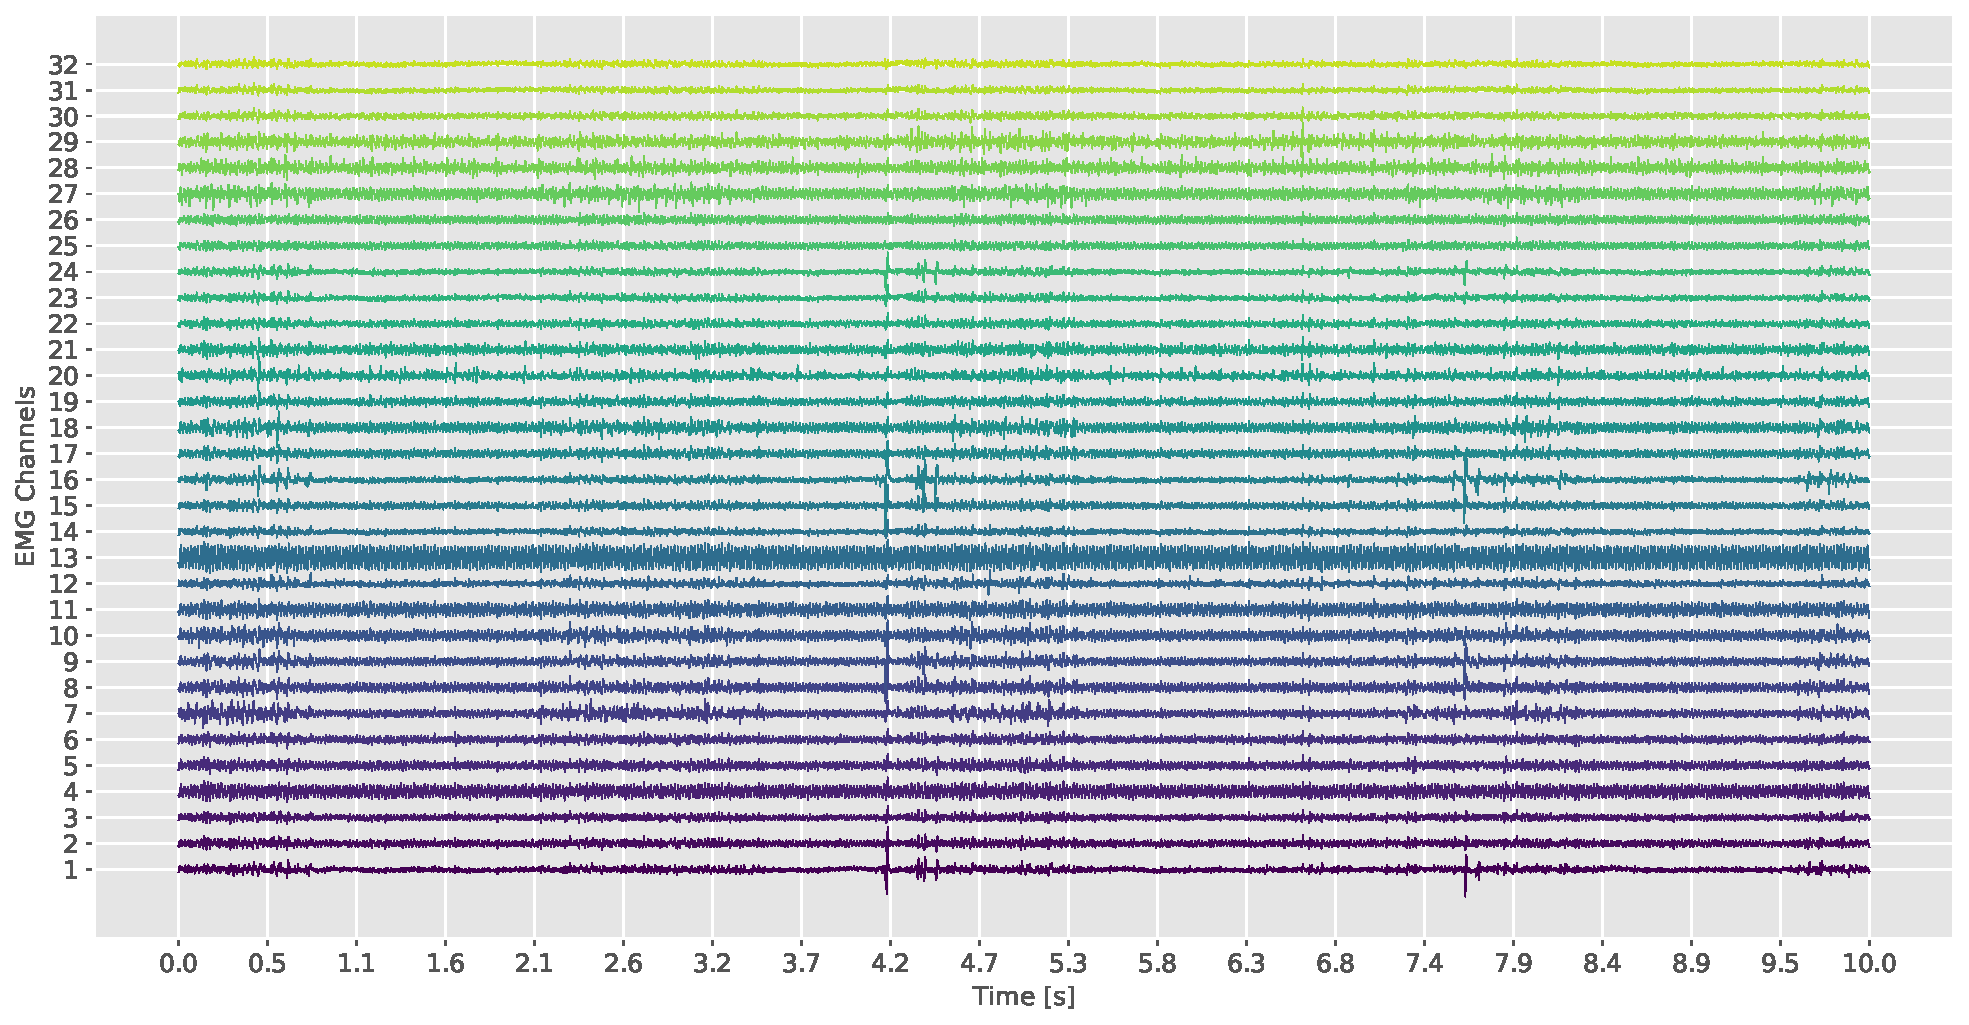
\includegraphics[width=1\textwidth,height=\textheight]{images/data_analysis/fingers/raw_data.pdf}
\caption{10 seconds of raw 32-channel EMG data taken during a minimal
finger flexion trial. Note that some channels include a nontrivial
amount of line noise. This noise will be drastically reduced through
changes being made in the next recording hardware revision which include
shielding, shorter cables, and better cable routing. Note that some
channels (e.g.~channel 24) show very low noise and putative single motor
unit action potentials can be seen on many
channels.}\label{fig:raw_data}
}
\end{figure}

To preprocessing the data, simple filtering and rectifying were applied,
as is commonly done in the
literature\textsuperscript{\protect\hyperlink{ref-sangerBayesianFilteringMyoelectric2007}{35}--\protect\hyperlink{ref-sussillo2015}{38}}.
As shown in \cref{fig:preprocessing_steps}, here we apply highpass
filtering at 40Hz to remove any low-frequency oscillations and DC
offsets, rectification and lowpass filtering at 5Hz to extract what is
typically associated with a force readout of the EMG signal in the case
that electrodes are positioned over the belly of a single muscle. These
filter parameters were chosen by visual comparison across a range of
values. While these preprocessing steps are in accordance with the
literature and yield a signal with frequencies on a behavioral timescale
though, as discussed in \cref{sec:next_steps}, preprocessing of raw EMG
signals is an area worth investigating the development and application
of more advanced methods.

\begin{figure}
\hypertarget{fig:preprocessing_steps}{%
\centering
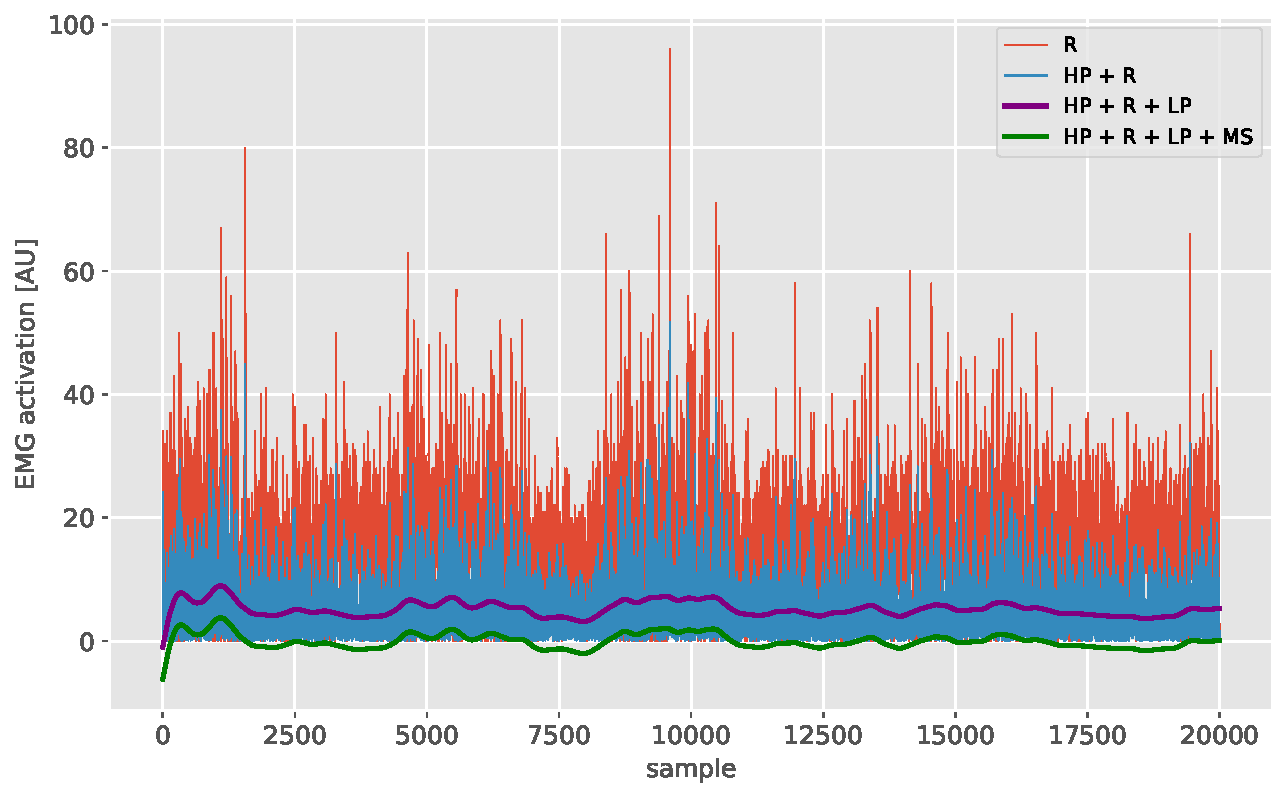
\includegraphics[width=1\textwidth,height=\textheight]{images/data_analysis/fingers/preprocessing_steps.pdf}
\caption{Data from a single trial showing each step of preprocessing.
The prototype preprocessing pipeline is highpass at 50Hz, rectification,
and lowpass at 5Hz. The within-trial, per-channel means are subtracted
from each trial. This matches what is typically done in the literature
to find a correlate of intended
force\textsuperscript{\protect\hyperlink{ref-sangerBayesianFilteringMyoelectric2007}{35}--\protect\hyperlink{ref-sussillo2015}{38}}.
There is significant room for improvement on this workflow, as discussed
in the text.}\label{fig:preprocessing_steps}
}
\end{figure}

\hypertarget{open-loop-finger-recordings}{%
\subsection{Open-loop Finger
Recordings}\label{open-loop-finger-recordings}}

In our first preliminary experiment, a single subject produced flexions
and extensions of each finger in the recording setup without any kind of
artificial feedback. One trial was collected per finger movement in
three blocks per session and one session per day over five days for a
total of fifteen trials per finger movement. The purpose of this
experiment is to determine the robustness over trials and sessions of
EMG features for a simple low-contraction movement, as well as to
determine the level of noise and artifacts in the data. Such baseline
measurements are important to properly decompose variability due to
electrode placement and exogenous noise from behavioral and
physiological variability in order to ensure reproducibility of our
results. Additionally, this baseline task may prove useful as a
benchmark for later tasks in terms of testing analysis and decomposition
techniques. A plot of all 32 channels for a single trial after
preprocessing is shown in \cref{fig:preprocessed_data}.

\begin{figure}
\hypertarget{fig:preprocessed_data}{%
\centering
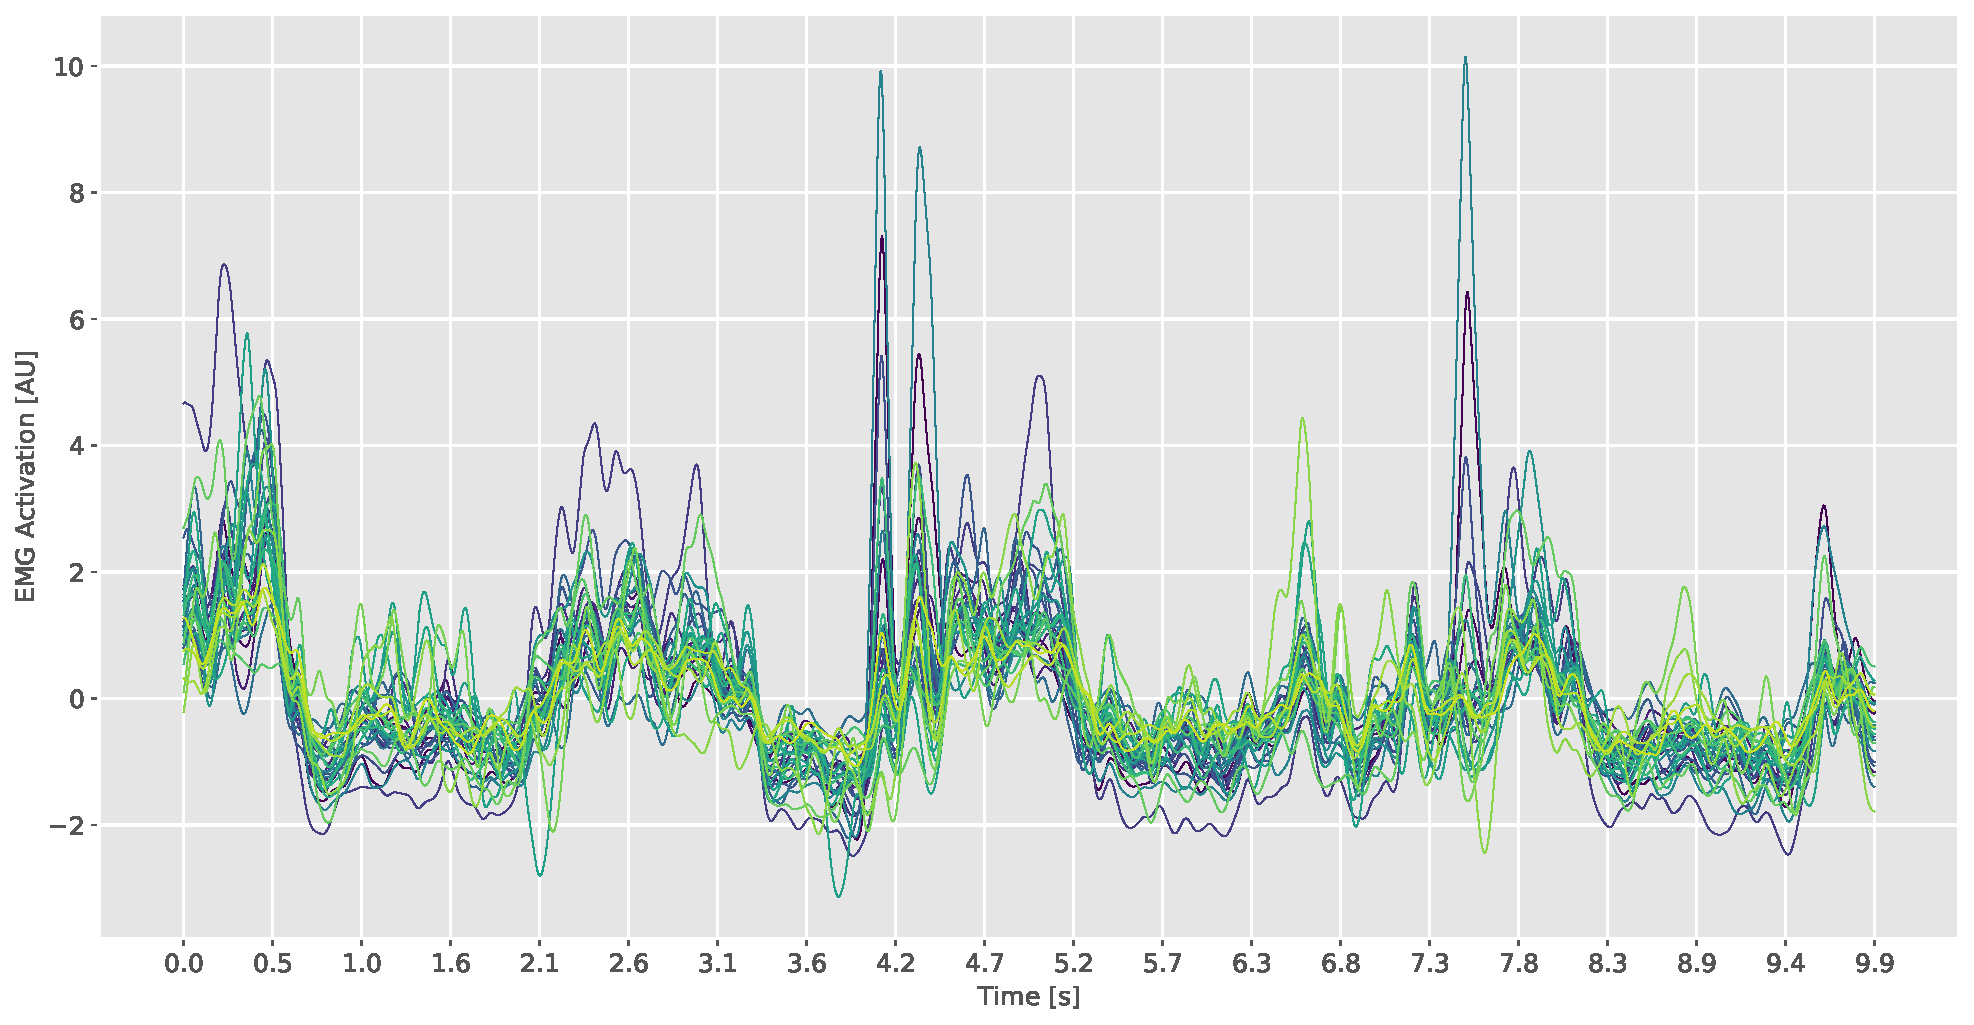
\includegraphics[width=1\textwidth,height=\textheight]{images/data_analysis/fingers/preprocessed_data.pdf}
\caption{All channels of data from a single trial after preprocessing.
Note the difference in baseline for each channel. Ideally, each channel
has a clear baseline of no activity, as further discussed in the main
text.}\label{fig:preprocessed_data}
}
\end{figure}

We first asked whether PCA applied to each individual trial would
extract a single, high-variance component reflecting the dimensionality
of the behavior. Since each finger movement is intuitively one
dimensional, we predict that PCA would find a single high-variance
component when run on each individual trial. As shown in
\cref{fig:PCA_variances}, this is generally the case, though there are
some outlier trials. After inspecting these outlier trials, it is likely
that the subject moved multiple fingers in these trials counter to the
experimenter's instruction.

\begin{figure}
\hypertarget{fig:PCA_variances}{%
\centering
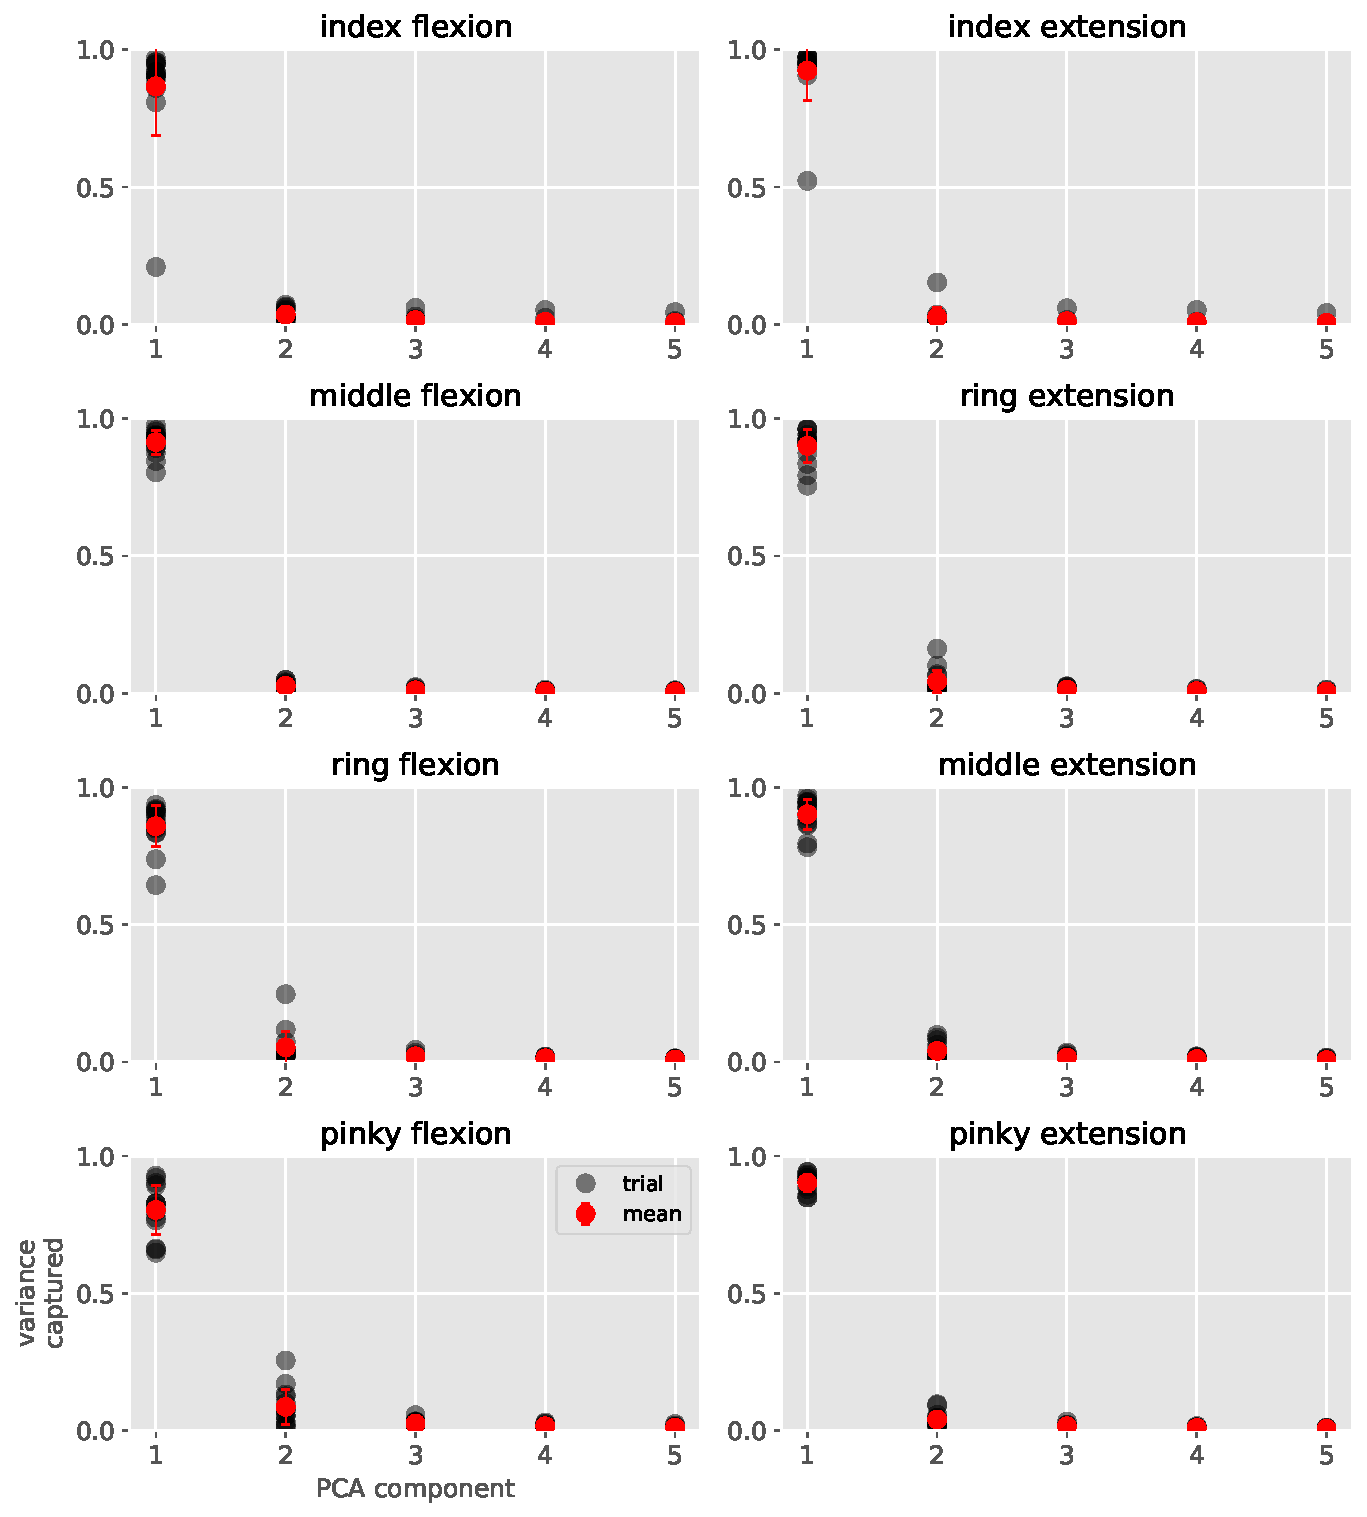
\includegraphics[width=1\textwidth,height=\textheight]{images/data_analysis/fingers/PCA_variances.pdf}
\caption{Fraction of variance captured by the top 5 principle components
for trials of single finger extensions and flexions. PCs were computed
for individual trials. Trials were recorded from one subject for 10s
each trial with finger movement frequency approximately 1Hz. Three
blocks each with one trial per finger movement were recorded per day for
5 days for a total of 15 trials per finger. Electrodes were not removed
between blocks but were removed between days. Each trial displays a
single high-variance PC component.}\label{fig:PCA_variances}
}
\end{figure}

We next asked, since each trial appeared to be dominated by a single
principle component, whether this top component was stable across trials
and across days. If the top component is stable, it implies that the
recording apparatus is robust to electrode movement between sessions.
The top components for each movement after running PCA on each trial are
shown in \cref{fig:PCA_components}. While it is not typical to run PCA
on individual trials, for the purpose of visually inspecting the PCA
weights over EMG channels it is used here.

\begin{figure}
\hypertarget{fig:PCA_components}{%
\centering
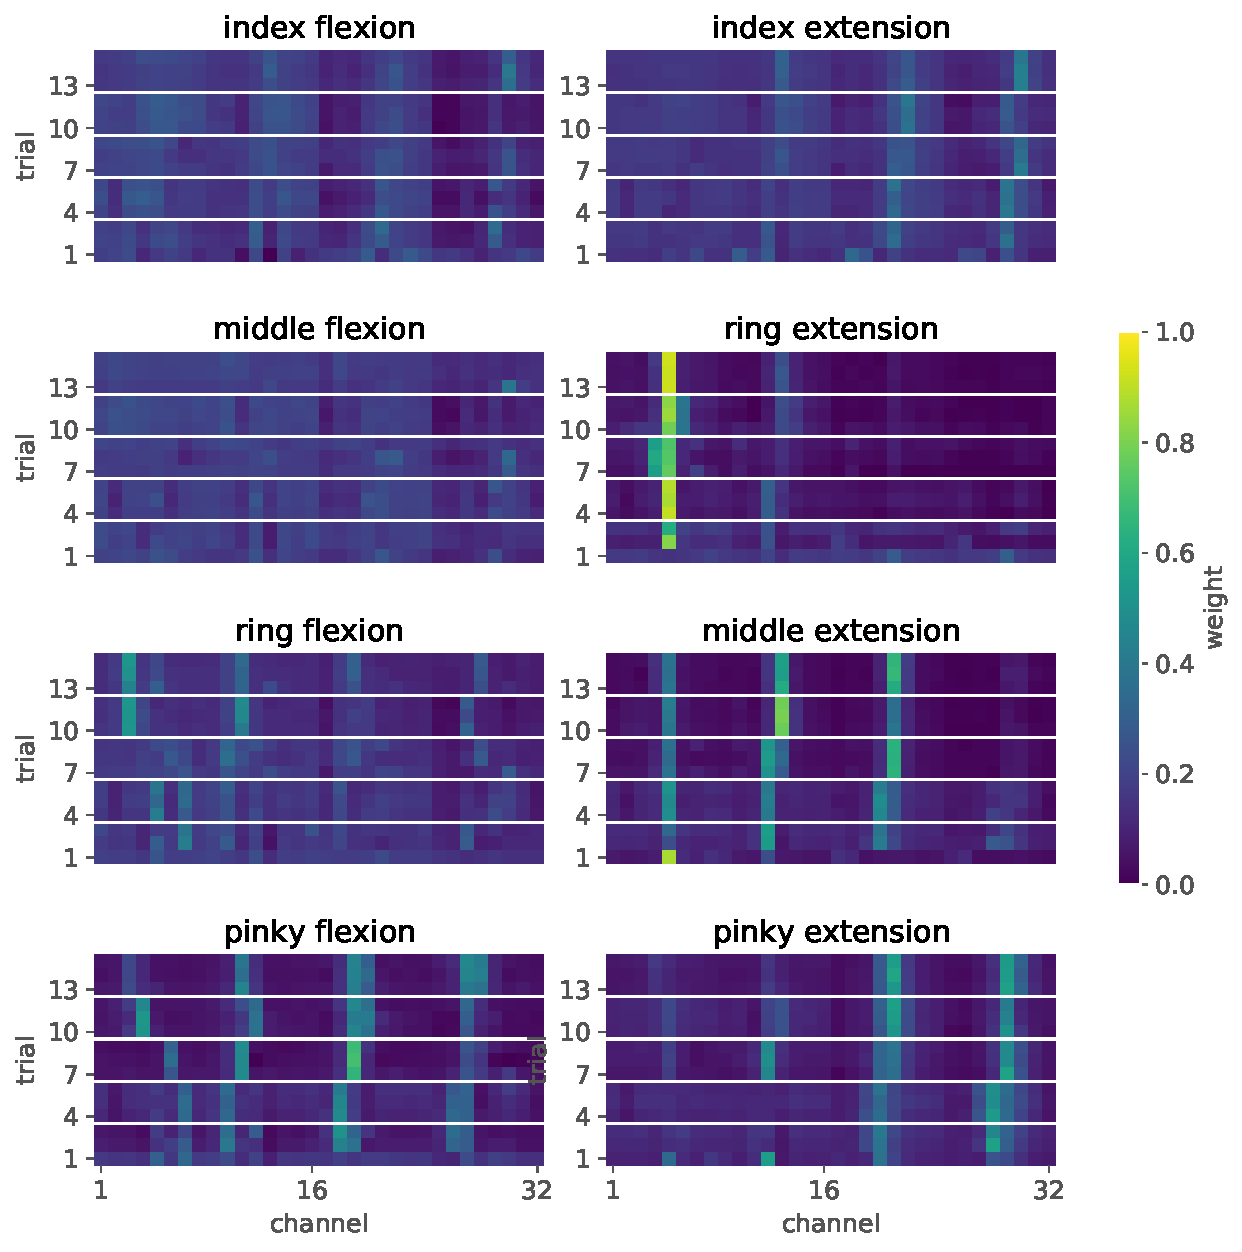
\includegraphics[width=1\textwidth,height=\textheight]{images/data_analysis/fingers/PCA_components.pdf}
\caption{The top principle component from each single finger movement
trials plotted as weights across channels. PCA was computed for each
trial individually. White horizontal lines show breaks between days when
electrodes were removed and reapplied. Each trial's top component is
relatively stable across trials and across days, though there is drift
and dropout of weights. Measures to increase cross-session stability are
discussed in the main text. Movements appear to vary between strong
localization on single channels and broad activation across
channels.}\label{fig:PCA_components}
}
\end{figure}

The results here suggest that, at least up to linear decompositions, the
features of low-contraction movements is relatively robust across
sessions. As discussed in \cref{sec:next_steps}, we will construct more
reliable means to place electrodes on subjects' forearms to further
increase repeatability. Another aspect of these results is our
assumption subjects are producing the same contraction each time they
move their finger, and at the same contraction level. That is, we assume
they are recruiting the same motor units each movement. This may not be
the case, and constructing new analyses which infer motor unit
activations may be useful to mitigate this issue.

\hypertarget{center-hold-reach-out-task}{%
\subsection{Center-hold Reach-out
Task}\label{center-hold-reach-out-task}}

In this task, the 32-dimensional EMG electrode activity vector is mapped
to a 2D force acting on a point mass shown on the screen. The mapping
\(M\in\mathbb{R}^{2x32}\) maps 8 ``columns'' each consisting of 4
electrodes placed in a line down the length of the forearm each to one
of 2D root of unity. Each column of electrodes is thus mapped to one of
8 two-dimensional force vectors. In this experiment, the point mass has
zero inertia and zero friction and as such displays a direct, though
redundant, readout of the EMG signal. The task asks the subject to reach
one of 32 equally spaced targets on each trial. Subjects must hold in
the center of the task space for a designated period of time, after
which the target appears. Subjects then have a time window reach the
target. Data from one subject was recorded for three blocks in one
session. Each block consisted of 32 trials, one per target in a
randomized order.

The mapping between EMG and task space \(M\) can be written as

\[
M = \begin{bmatrix}\tilde{M} & \tilde{M} & \tilde{M} & \tilde{M}\end{bmatrix}
\]

where \(\tilde{M}\) consists of 8 equally spaced directions, one for
each ``column'' of the 4 EMG electrode bands around the subject's arm:

\[
\tilde{M} =
\begin{bmatrix}
0  & 0.71  & 1   & 0.71   & 0  & -0.71  & -1  & -0.71 \\
1  & 0.71  & 0  & -0.71  & 1   & -0.71   & 0   & 0.71
\end{bmatrix}
\]

A graphic showing the mappings from electrodes to force directions is
shown in \cref{fig:columns}. While there are 8 possible force vectors
the subject can modulate by controlling the electrode activity on each
of her 8 columns, the EMG mapping is ultimately a projection onto the 2D
plane. Since the EMG signal is nonnegative, the subject could
technically modulate just four modes of electrode activity, the minimum
number needed to span the task space, to reach all 32 targets. This
mapping was chosen in order to provide a simple starting point to
explore the virtual EMG task. There are no added environmental dynamics,
only a redundant readout of force, and the signal is processed online in
the same manner as in the offline analyses. This task or a variant we
think can serve as a foundation upon which we can build more complex
mappings and virtual environments. Task space trajectories from each
block are shown in \cref{fig:trajectories}. The fraction of trials
resulting in hold timeouts, reach timeouts, and target hits are shown
over blocks in \cref{fig:hit_fraction}.

\begin{figure}
\hypertarget{fig:columns}{%
\centering
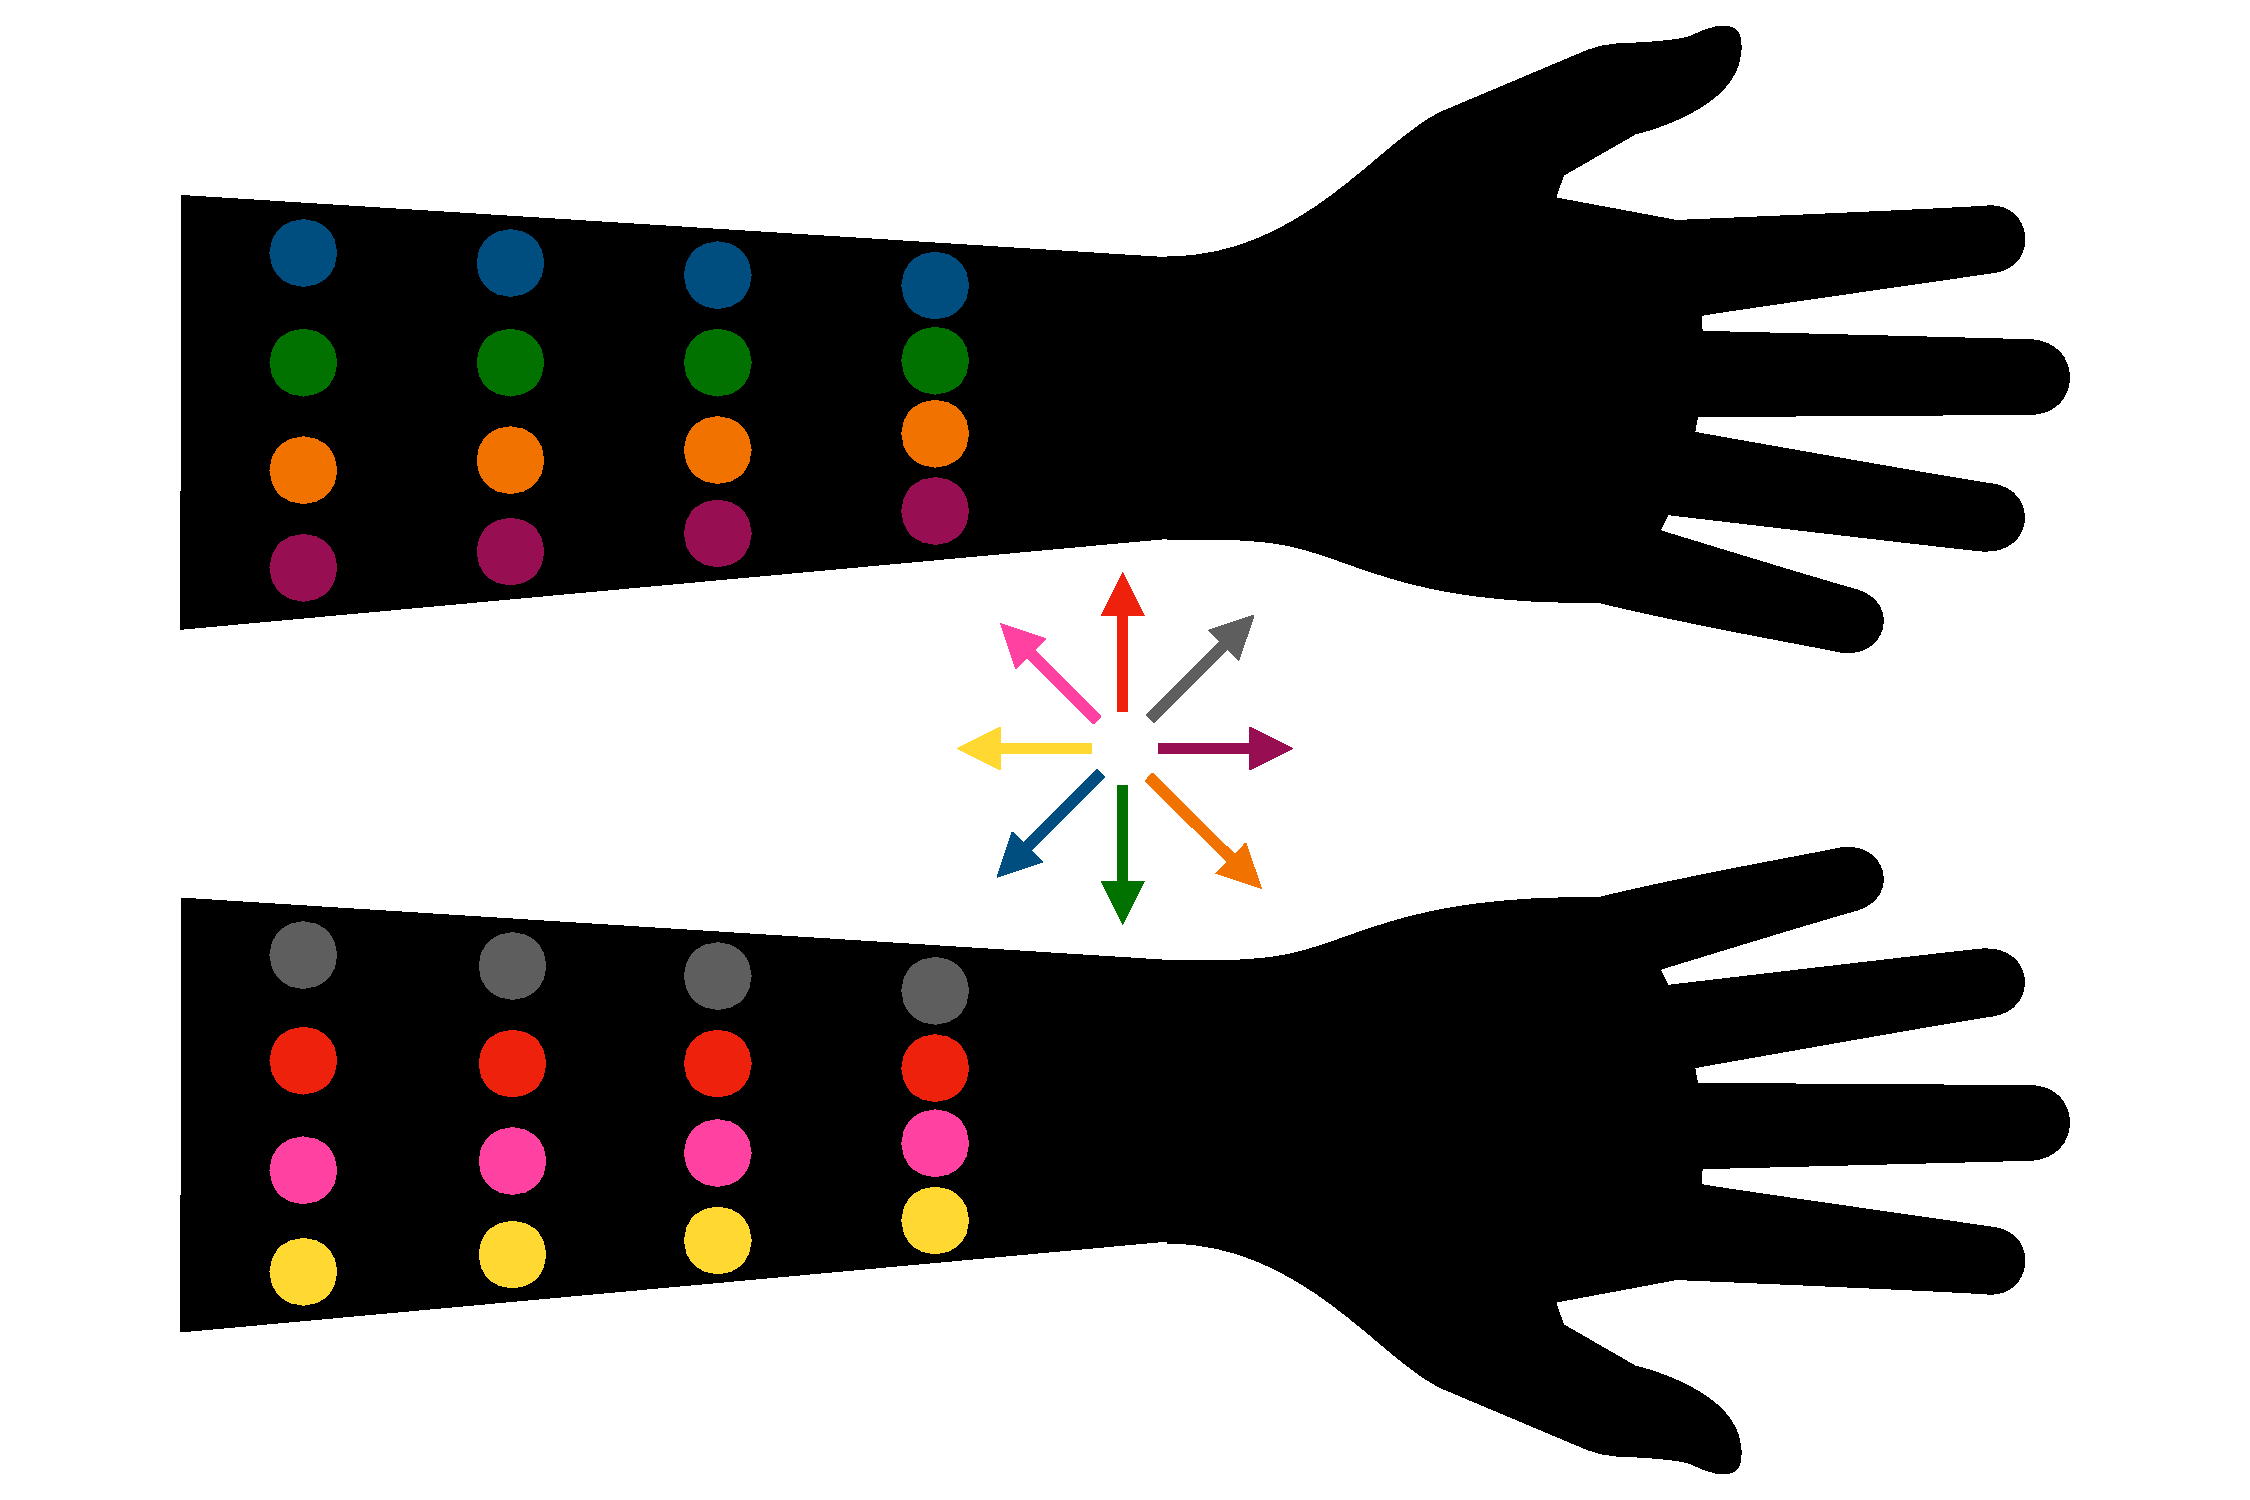
\includegraphics[width=0.7\textwidth,height=\textheight]{images/hardware/columns.pdf}
\caption{Graphic showing the mapping between electrodes in the
32-channel center-hold reach-out experiment to eight 2D force directions
in the virtual task space. Each of the eight columns consists of four
electrodes each mapped to the same force direction (denoted with
matching color) acting on a virtual point particle.}\label{fig:columns}
}
\end{figure}

\begin{figure}
\hypertarget{fig:trajectories}{%
\centering
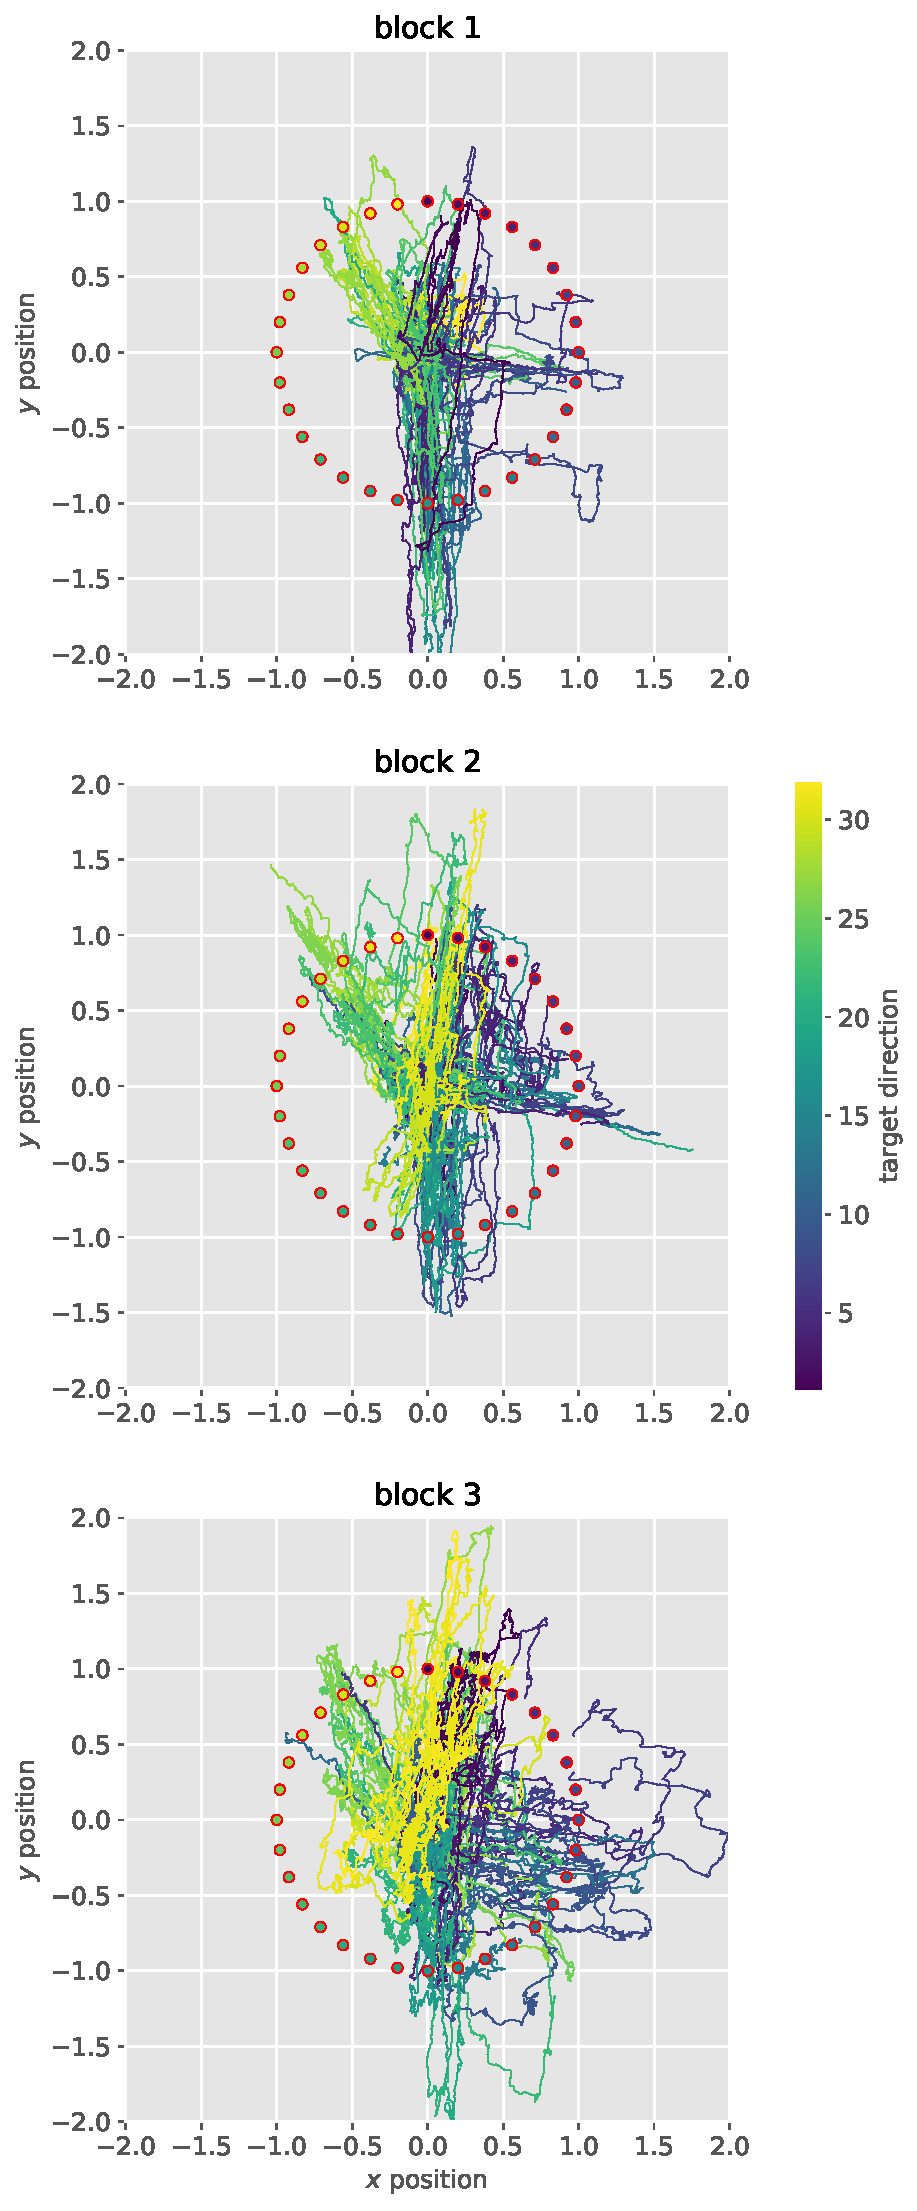
\includegraphics[width=0.6\textwidth,height=\textheight]{images/data_analysis/center_hold/trajectories.pdf}
\caption{Point mass position trajectories in two-dimensional task space
during the center-hold, reach-out task with 32 targets spaced evenly
around the unit circle (shown with red borders). Color corresponds to
target numbers, with target zero located at (0,1). Target order was
randomized. Training was conducted over 3 blocks each with 32 trials, 1
trial per target.}\label{fig:trajectories}
}
\end{figure}

\begin{figure}
\hypertarget{fig:hit_fraction}{%
\centering
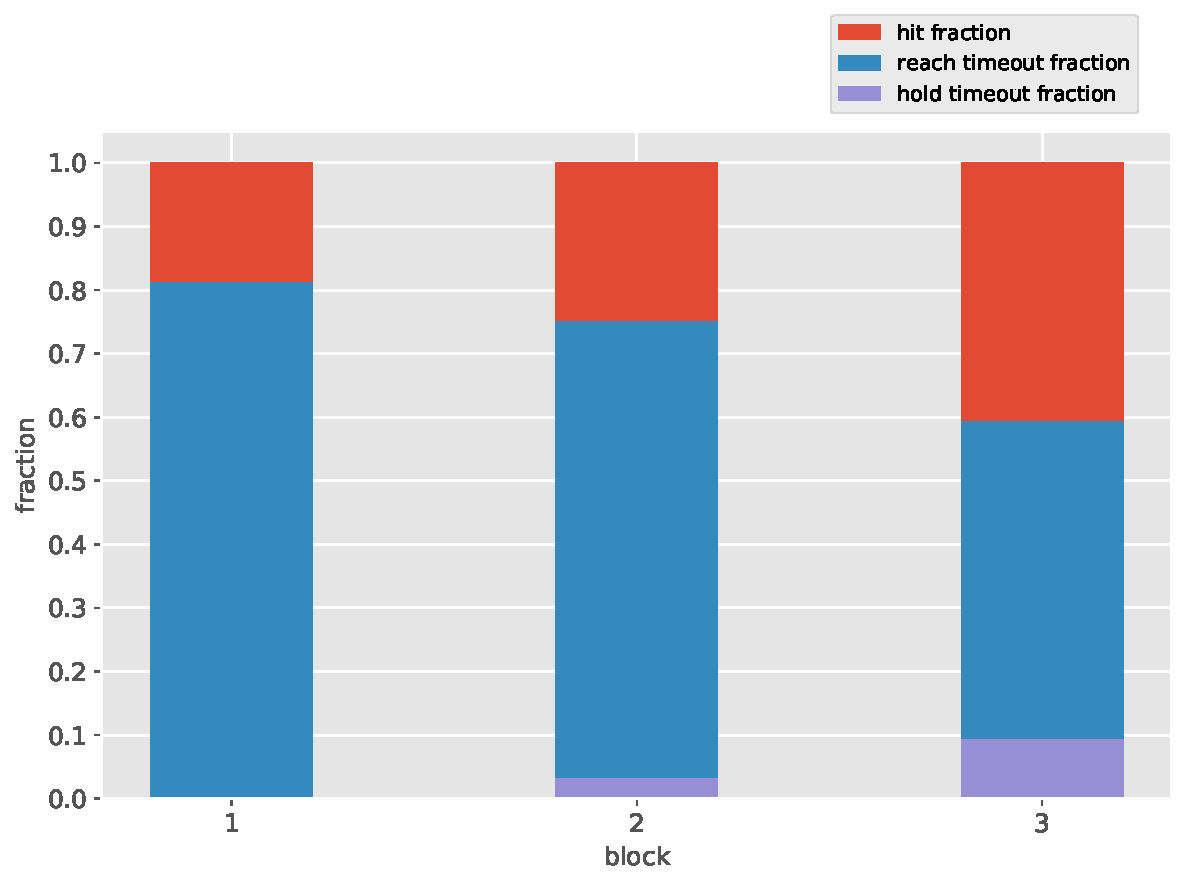
\includegraphics[width=0.7\textwidth,height=\textheight]{images/data_analysis/center_hold/hit_fraction.pdf}
\caption{Fractions of trial outcome types for each block of the
center-hold, reach-out task. Hit fraction increases on each trial,
suggesting the beginnings of task learning. Hold timeout failure
increases over trials as well, perhaps suggesting increased baseline
excitation of muscles during the hold period. Part of learning to
activate certain muscle modes is learning to inhibit
others.}\label{fig:hit_fraction}
}
\end{figure}

In this task, the subject's first goal is to interact through the
mapping \(M\) and learn the consequences of various motor activations.
That is, they must internalize a model of the virtual environment, what
might be called a system identification problem. Subjects must collect
data containing motor outputs and their sensory consequences. To do
this, they must explore the space of activity. We predict that over
trials, subjects' EMG activities over channels will become more varied
as they attempt new movement patterns to achieve their twin goals of
learning to move in this new environment and reaching the target.
Running PCA on each individual trial's EMG time series, we hypothesize
that initially we will see multiple components share signal variance as
subjects explore. Eventually, we would expect to see a decrease in this
measure of movement complexity a subjects hone their reaching skill.
Trial-level PCA component variance fractions are shown in
\cref{fig:PCA_trial_variance}. We find an initial decrease in the top
component's variance fraction, though we expect many more trials will be
needed to see skill acquisition in the form of a dominant movement mode
per trial.

\begin{figure}
\hypertarget{fig:PCA_trial_variance}{%
\centering
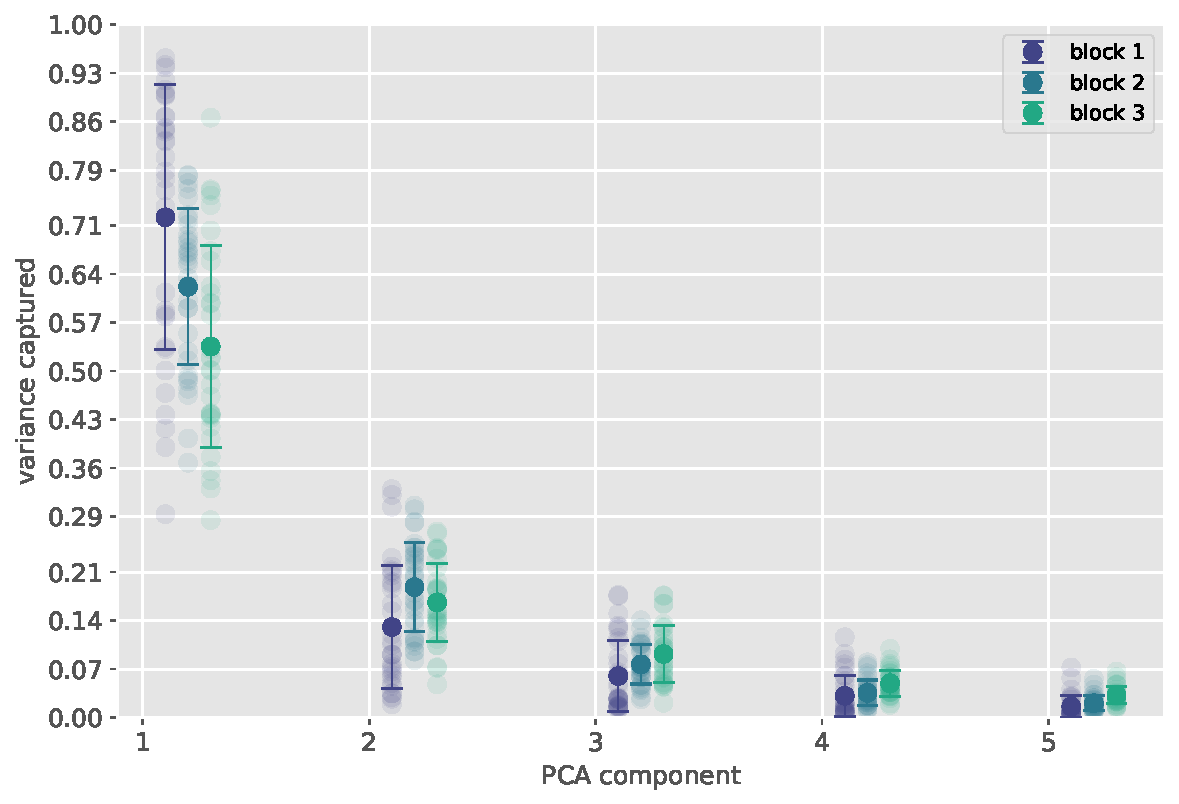
\includegraphics[width=0.7\textwidth,height=\textheight]{images/data_analysis/center_hold/PCA_trial_variance.pdf}
\caption{Fraction of variance captured by the top five principle
components when PCA is run on the EMG time series' of individual trials
of the center-hold, reach-out task. Error bars are standard deviation.
Over blocks, we see a slight decrease in the mean of the top component's
variance fraction, though with high variance. This may suggest greater
exploration within-trial, as less variance is captured by a single
component over blocks, though it could reflect more varied dynamics
across trials as the subject discovers new, task-relevant
activations.}\label{fig:PCA_trial_variance}
}
\end{figure}

We might model this task as the subject selecting an EMG signal \(x\)
which minimizes the distance between a target position \(b\) and the
projection of the EMG signal through the mapping \(M\) as well as
minimizes the norm of \(x\) in order to conserve metabolic energy. This
optimization can be written as a regularized least squares problem:

\[
\min_x\frac{1}{2}||Mx - b||^2_2 + \frac{\lambda}{2}||x||_2^2.
\]

This problem is known to have a unique minimum for \(\lambda>0\) which
is an approximation \(Mx\approx b\) regardless of the shape or rank of
\(M\). This implies that the subject, if they are biophysically capable
to do so, will learn distinct motor outputs for each target rather than
reusing modes for multiple targets with different activation levels.
That is the subject will, over time, learn to fractionate their muscle
output to reach their goal in order to minimize effort. For instance, to
reach the the target at position \((1,0)\) in Cartesian coordinates, the
subject could activate a bespoke activity mode and activate a
combination of two or more modes for targets at \(\pm45^\circ\) from
this central target. If this is the case, the model predicts that the
dimensionality of the EMG signal will increase over the course of
training as the subject learns to construct bespoke activity modes for
each target.

In \cref{fig:PCA_concat_variance} we compute PCA on the concatenation of
all trials within blocks for which we predict an increase in the number
of dominant EMG modes as subjects learn multiple movements to reach
individual targets. We expect subjects to, over time, develop some
number of bespoke movement modes to activate independently and as a
composition to reach each target. We find a suggestion of this idea in
the data with our basic PCA analysis. More trials, session, and subjects
will be required to explore this idea, and we are investigating
probabilistic measures of signal complexity such as entropy to formalize
this hypothesis. One direction might be to further define this task a
regularized regression with different regularization terms chosen
normatively for different sections of the learning and control process,
and fitting data to these predictions. For instance, early in training
subjects may not optimize for target accuracy as much as for signal
sparsity, whereas later in learning subjects may optimize for target
accuracy and output signal magnitude.

\begin{figure}
\hypertarget{fig:PCA_concat_variance}{%
\centering
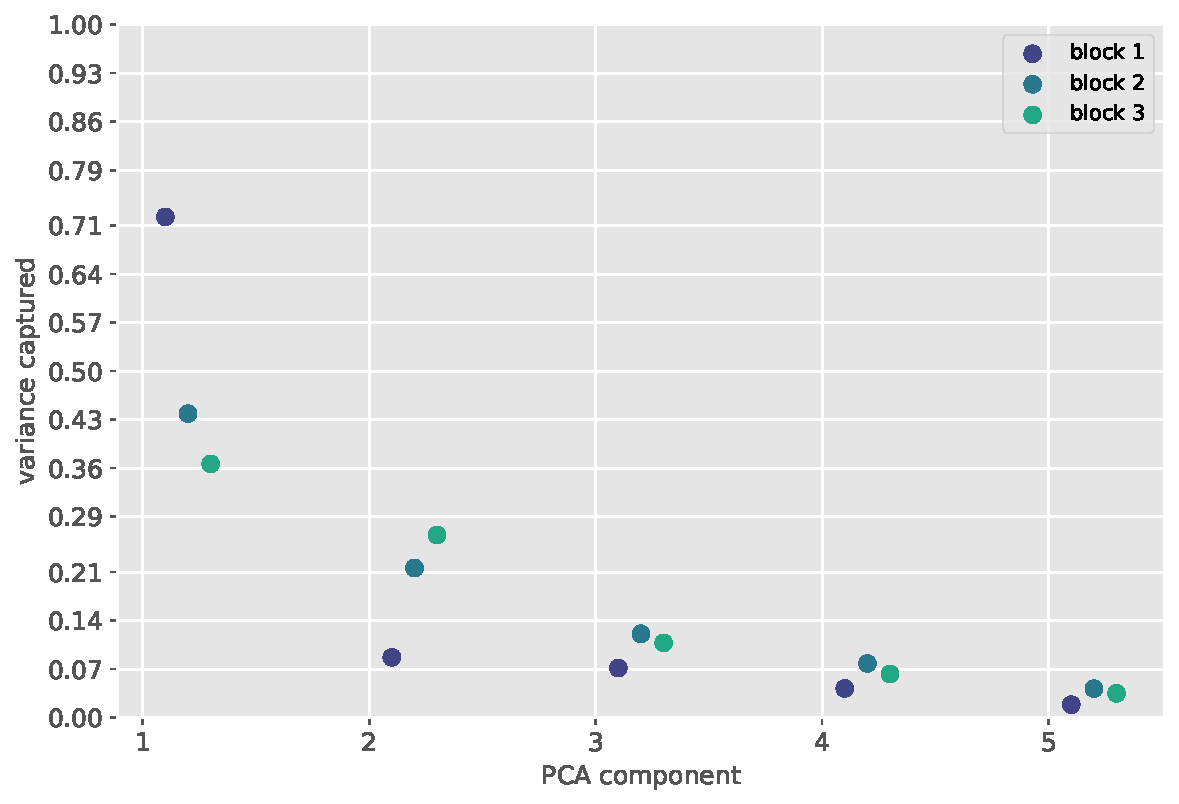
\includegraphics[width=0.7\textwidth,height=\textheight]{images/data_analysis/center_hold/PCA_concat_variance.pdf}
\caption{Fraction of variance captured by PCA computed on concatenated
EMG time series concatenated over trials. Over blocks, we see variance
shifting from the top component to other components. We hypothesize that
across learning we would see the development of bespoke modes used in
combination to reach individual targets. This would predict an increase
in the complexity of the EMG time series over learning. Here we see
suggestions of this prediction.}\label{fig:PCA_concat_variance}
}
\end{figure}

\clearpage

\hypertarget{sec:theory}{%
\section{Preliminary Theory}\label{sec:theory}}

\begin{quote}
\emph{An interesting open question is how to relate trial-to-trial
dynamics of learning to asymptotic predictions regarding optimal
adaptation.}

--- Todorov, \emph{2007}
\end{quote}

\hypertarget{optimal-feedback-control}{%
\subsection{Optimal Feedback Control}\label{optimal-feedback-control}}

The optimal feedback control framework remains the strongest normative
model of human movement control. The first step of our theoretical work
is to build from the simplest optimal feedback control models, working
towards constructing our own variants of such models in order to capture
aspects of our experimental findings. The first model we will
investigate is the fully-observable, discrete-time, infinite-horizon
linear quadratic regulator (LQR) problem with additive Gaussian noise.
Given a state \(x\in{\mathbb{R}^n}\) and an control input
\(u\in{\mathbb{R}^m}\), the state evolves in discrete time according
linear dynamics

\[
x_{t+1} = Ax_t + Bu_t + w_t
\]

where \(w_t\sim\mathcal{N}(0,\mathbb{I})\) The LQR problem is to find a
sequence of controls \(u_t\) which minimize a cost \(J\)

\[
J = \mathbb{E}\sum_{t=0}^{\infty}{x_t^TQx_t + u_t^TRu_t}
\]

according to some chosen state and control cost parameters \(Q\) and
\(R\). The optimal cost-to-go or state value function for the problem is

\[
V_t(x) = \min_{u}\left[{x_t^TQx_t + u_t^TRu_t + V_{t+1}(Ax+Bu)}\right].
\]

The optimal control law \(L\) which solves this problem is linear
function in the state

\[
u_t^*(x) = -Lx.
\]

This control law is found through iterating a Riccati equation involving
\(A\), \(B\), \(Q\), and \(R\) to find the optimal \(V\) which is a
quadratic function in state. There is a functional relationship between
\(V\) and \(L\) that can be derived algebraically.
\cref{fig:control_field} shows simulated trajectories of the
infinite-horizon problem from random initial positions. The vector field
depicts the two-dimensional control vector. In this example, the model
describes a second-order point mass dynamical system where the control
input acts as a force on the particle. The state vector \(x\) contains
two dimensions each of position, velocity, and force of the particle,
each updated via Euler integration. \cref{fig:cost_field} shows the same
simulated trajectories of the point mass atop the quadratic value
function. The goal state in these simulations is (0.5,0.5). Note that
there are many free dynamics parameters in such simulations within \(A\)
and \(B\) which drastically alter the resulting simulations. The values
here were chosen to match the motor control literature.

\begin{figure}
\hypertarget{fig:control_field}{%
\centering
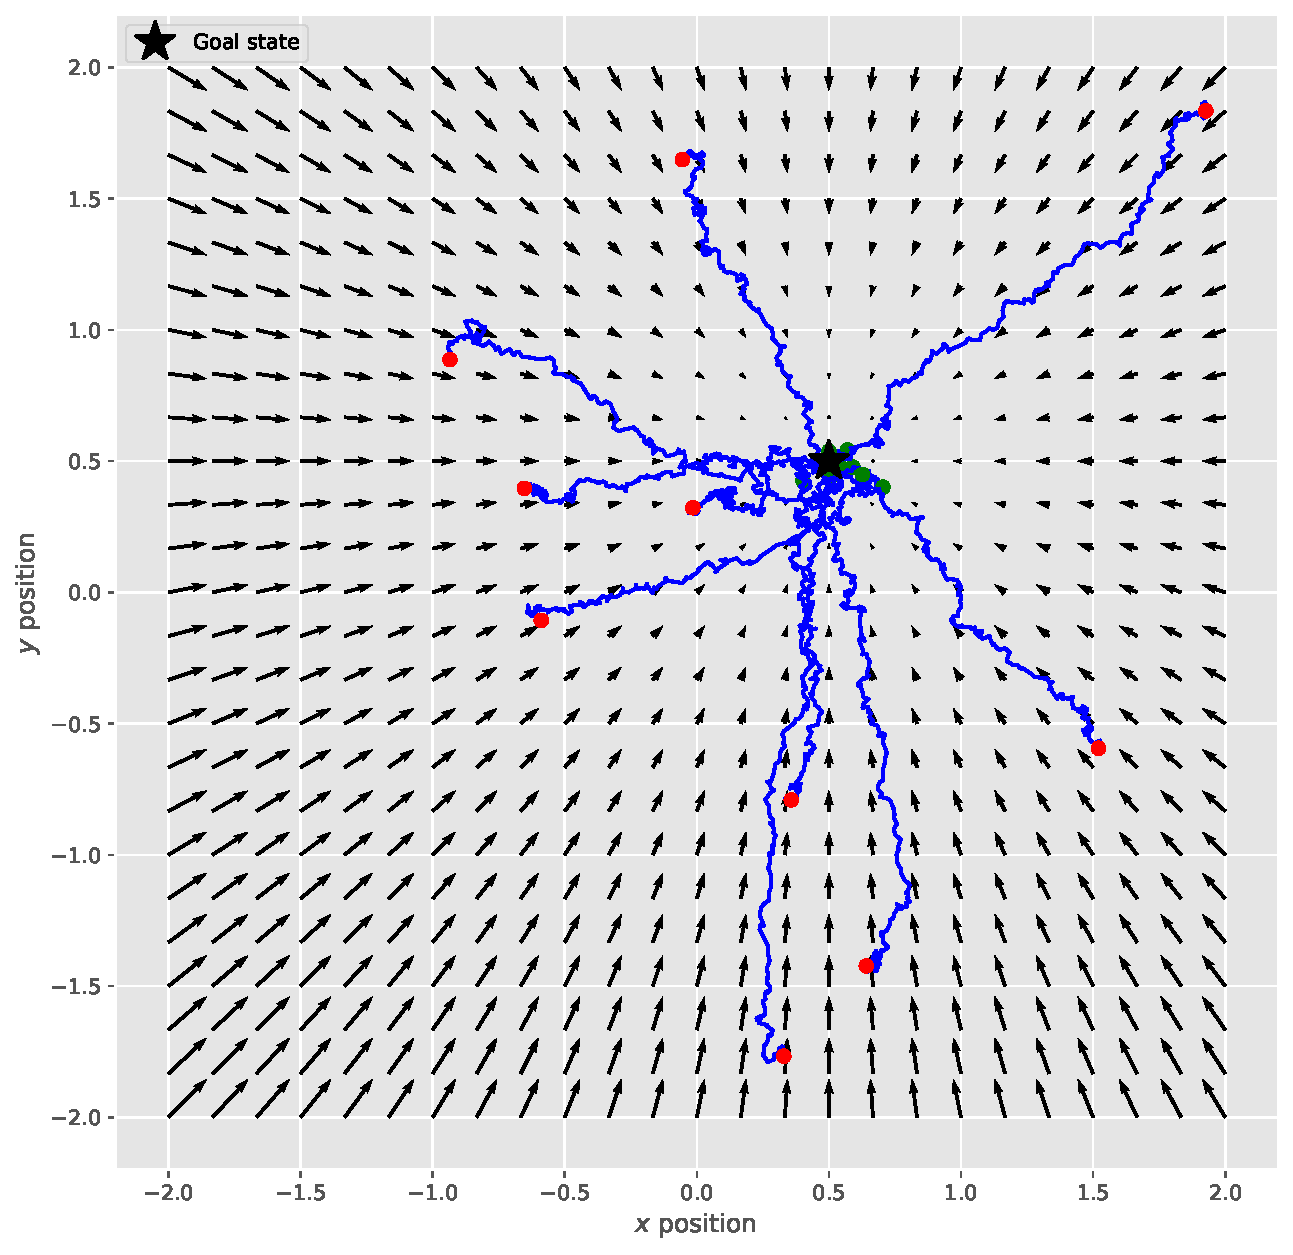
\includegraphics[width=0.7\textwidth,height=\textheight]{images/simulations/control_field.pdf}
\caption{Simulation of trajectories from uniform random initial
positions for the simplest LQR controller. The diffusions are controlled
such that their inputs are proportional to the positional error. The
plain LQR controller is invariant (up to a translation) to the goal
state, as explained in the text. Here the goal state is (0.5,0.5)
denoted by a white star. red circles denote the initial position of the
trajectory and green circles denote the endpoint after 200 increments.
Arrows show the state-dependent control signal (force) vector
\(u^T = [f_x,f_y]\).}\label{fig:control_field}
}
\end{figure}

\begin{figure}
\hypertarget{fig:cost_field}{%
\centering
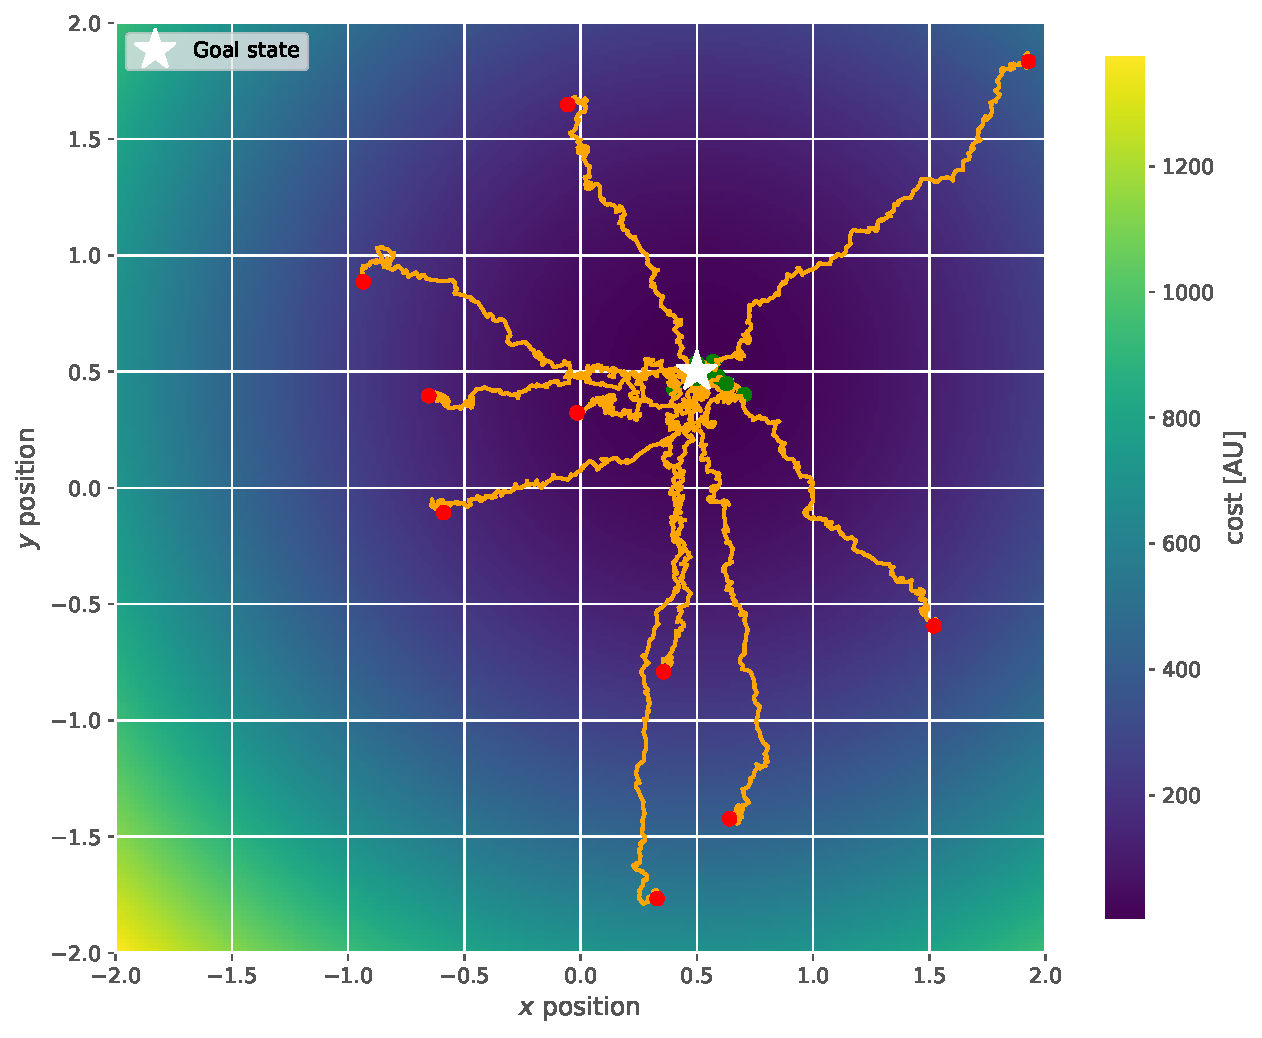
\includegraphics[width=0.7\textwidth,height=\textheight]{images/simulations/cost_field.pdf}
\caption{The same trajectory simulations as in \cref{fig:control_field}
atop the quadratic cost field.}\label{fig:cost_field}
}
\end{figure}

Assuming that the original system is controllable and stabilizable, the
linear optimal control problem is a matter of trading off eigenvalues of
the closed loop system which drive the steady-state error of the system
to 0 under the control cost. This system can be made to drive to a given
target \(x^*\) by feeding back evolving the dynamics in terms of target
error \(|x-x^*|\) or by augmenting the state vector with terms which
compute this error implicitly. These yield identical solutions for the
control law, the latter typically being more convenient. The implication
of this is that only one control law is required for the problem with a
point target in the state space. If the problem were to model human
movement, it might be said that we only require the internalization of a
single control law up to a translation in the target's desired state.
Only the error is required in this simple case. As discussed in
\cref{sec:next_steps}, variants of this basic model are more interesting
in that they do not display this target invariance.

\hypertarget{internal-model-adaptation-for-linear-quadratic-control}{%
\subsection{Internal Model Adaptation for Linear Quadratic
Control}\label{internal-model-adaptation-for-linear-quadratic-control}}

In experiments within the setup described in \cref{sec:experiment},
subjects are faced with a novel muscle-to-environment mapping that they
must ostensibly learn in order to achieve their goals. Here I
investigate the effects of approximating dynamics models within the LQR
framework. This short experiment is a first step in modeling how
subjects may use endpoint error in each trial to update or adjust their
internal approximations of the environment's dynamics.

Our state space is denoted \(x\) and our control space \(u\) where
\(dim(x) < dim(u)\). Each trial, we move from state \(x_0\) to x(N) in
\(N\) timesteps. Each trial, we have a goal state \(x^*\) and a
resulting endpoint error \(e_N = |x_N - x^*|^2\). We follow the same LQR
setup as defined in the previous section. We can write the controlled,
closed-loop system dynamics for the final time step \(N\):

\[
\begin{aligned}
x_N &= (A - BL)x_{N-1} = Cx_{N-1} \\
x_N &= Cx_{N-1} = C(Cx_{N-2}) \\
x_N &= C^Nx_0.
\end{aligned}
\]

where \(C^N\) might be called the trajectory dynamic. If the trajectory
dynamic \(C^N\) is an approximation to the true trajectory dynamic
\(C^{N*}\), we can use the error of a given trajectory to find an
incremental update. The error at the final time step \(N\) for trial
\(r\) is

\[
e(r) = |C^N(r)x_{0} - x^*|^2.
\]

This error may be due to several sources. Our internal dynamics model
\(A\) might have error relative to the true dynamic \(A^*\). Our control
gain \(L\) may be optimal relative to our internal model \(A\) but not
with respect to the true dynamic \(A^*\). Finally, we might have an
approximate model \(A\) and a suboptimal control gain \(L\). Note that
since this is still deterministic system, we have yet to include any
source of variability in state or control.

If we assume that our computation of the control gain \(L\) is optimal
for our approximate internal model \(A\) (we can compute a controller
given only our internal representation of the system dynamic being
controlled), we can use our endpoint error to derive a gradient descent
update for \(A\) on trial \(r\):

\[
A(r+1) = A(r) - \eta\frac{\partial{e(r)}}{\partial{A}}
\]

We might think about this as an internal simulation of trial \(r\)'s
trajectory, and a subsequent post hoc evaluation of the movement. To
compute \(\delta\), we must take the gradient with respect to A of the
error:

\[
\begin{aligned}
\frac{\partial{e(r)}}{\partial{A}} &= \frac{\partial{}}{\partial{A}}{|C^N(r)x_0 - x^*|^2}
\end{aligned}
\]

Since the gradient with respect to A is the same as the gradient with
respect to \(C\), we can compute the gradient with respect to C to find:

\[
% 2∑𝑁𝑘=1(𝑀𝑁𝑣−𝑤)𝑇𝑀𝑘−1𝑀𝑁−𝑘𝑣
\frac{\partial{e}}{\partial{A_{ij}}} = 2\sum_{k=1}^N\left[(C^Nx_0 - x^*)^TC^{k-1}\right]_i\left[C^{N-k}x_0\right]_j
\]

\cref{fig:gradient_descent} shows the LQR simulations across gradient
descent updates to the \(A\) matrix after it is corrupted by Gaussian
noise. Each trajectory is a single run of the LQR controlled for 200
time steps. The star shows the target state, the colored circles show
the endpoints of the trajectories. The red circle is the initial state.
The descent is converging in endpoint error in position, velocity, and
force dimensions of the state vector. Unfortunately, this optimization
alters the dynamics incompatibly. The routine is also very fragile to
parameter changes. This experiment highlights the difference in loss
landscapes between the optimal control problem and the gradient descent
simulated here. There are many directions for this work to proceed as
discussed in \cref{sec:next_steps}.

\begin{figure}
\hypertarget{fig:gradient_descent}{%
\centering
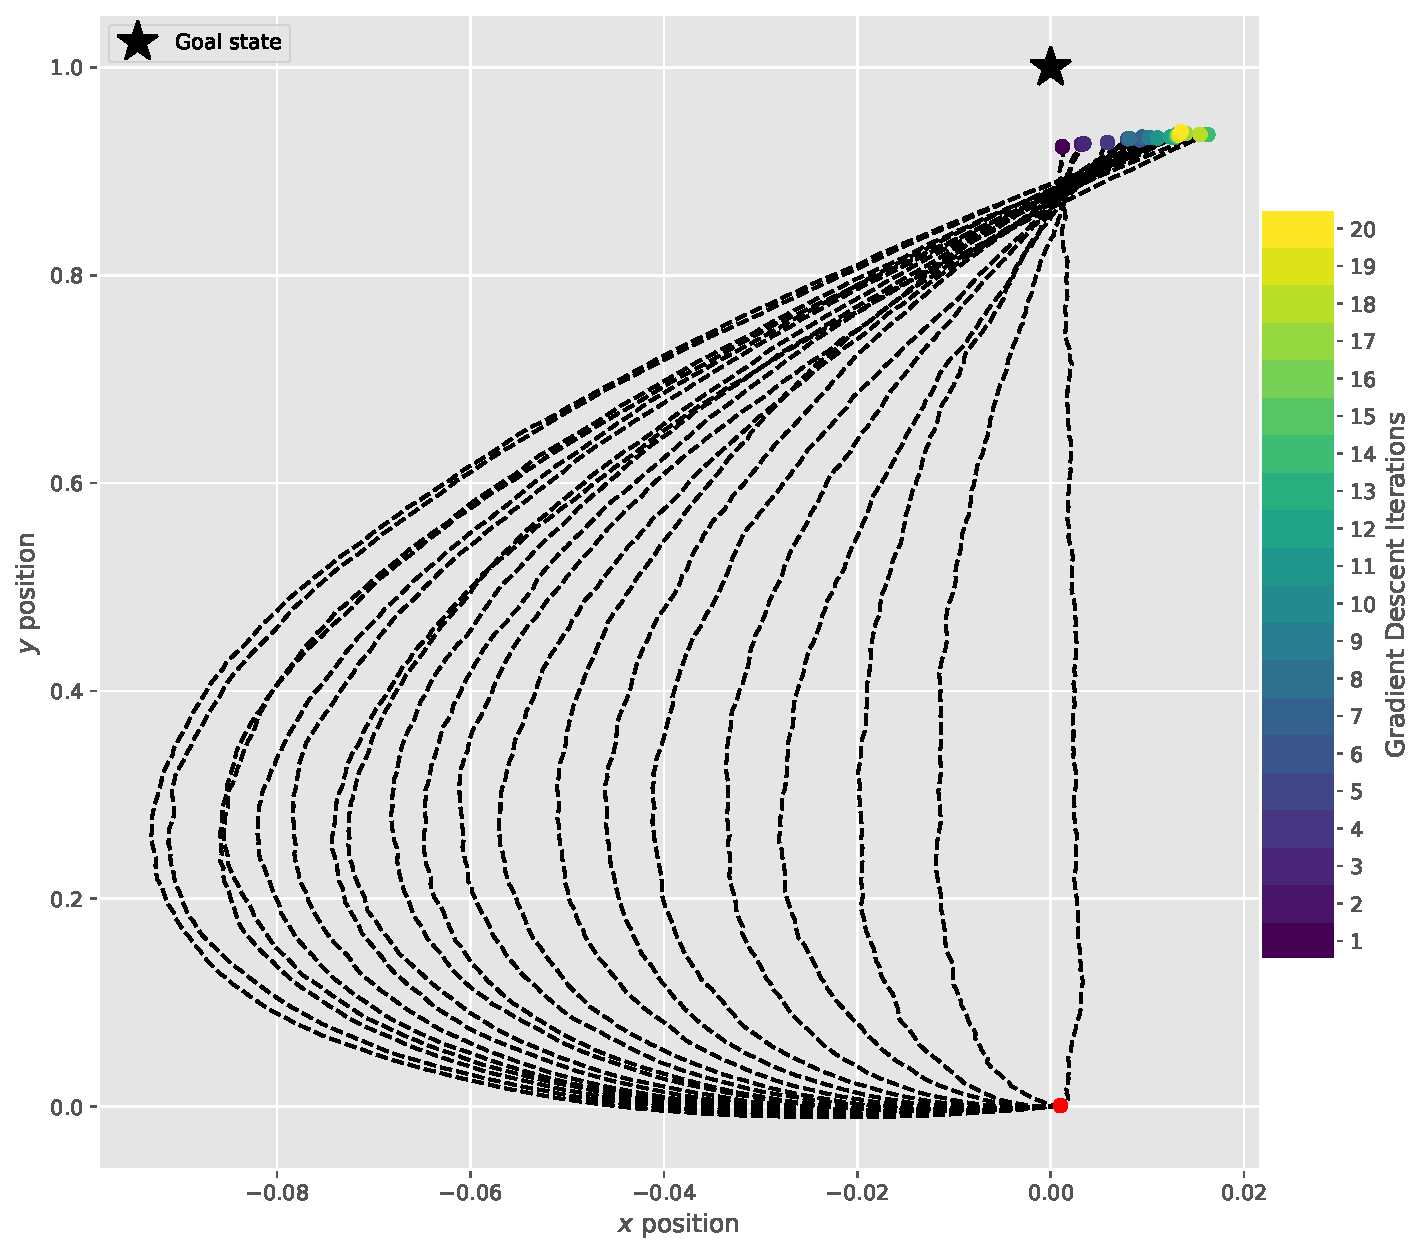
\includegraphics[width=0.75\textwidth,height=\textheight]{images/simulations/gradient_descent.pdf}
\caption{Iterations of gradient descent on the \(A\) matrix of an
infinite-horizon LQR where the original A is corrupted with Gaussian
noise. Each dotted line is a sampled trajectory using a recomputed
control gain with an updated \(A\) matrix. Red circles denote the
initial state, the star denotes the goal state, and the colored circles
denote the endpoints of each trajectory sampled at each iteration. Note
that the initial solution diffuses directly towards the target, and the
gradient updates for the dynamics model \(A\) alter this trajectory in a
nontrivial way. As discussed in the main text, the gradient descent is
optimizing for a different cost than the controller optimization, and
thus this divergence might be expected.}\label{fig:gradient_descent}
}
\end{figure}

\clearpage

\hypertarget{sec:next_steps}{%
\section{Next Steps}\label{sec:next_steps}}

\begin{quote}
\emph{When it comes to the problem of skilled movement, the algorithm is
simply not known.}

--- Wolpert \& Ghahramani, \emph{2000}
\end{quote}

\hypertarget{emg-hardware}{%
\subsection{EMG Hardware}\label{emg-hardware}}

Our preliminary data confirms the working principle of the setup and
highlights the next steps for producing quality datasets. This is in
accordance with the literature, where more advanced use of EMG is
emerging as an important tool in understanding the complexities of motor
computation\textsuperscript{\protect\hyperlink{ref-Hug2011}{39}}. Our
next steps are to build a new version of the EMG hardware doubling the
number of channels to 64 electrodes placed across the forearm and to
provide better hand constraints to ensure completely isometric
contractions. The next hardware version will also include investments in
shielding to provide proper noise mitigation. Most EMG in the literature
is smoothed and trial-averaged due to noise, but we are confident that
our records can be analyzed at the level of single trials, much like
recent developments in neural data
analyses.\textsuperscript{\protect\hyperlink{ref-churchlandNeuralPopulationDynamics2012a}{36},\protect\hyperlink{ref-churchlandNeuralVariabilityPremotor2006}{37}}

\hypertarget{eye-tracking}{%
\subsubsection{Eye Tracking}\label{eye-tracking}}

To completely close the loop in our experiments, we are working to
integrate pupil and gaze tracking to more closely follow the perceptual
aspects of our task. We hope to find correlations in line with the
literature dealing with active
learning\textsuperscript{\protect\hyperlink{ref-yangTheoreticalPerspectivesActive2016}{40},\protect\hyperlink{ref-huangActiveLearningLearning2008}{41}}.

\hypertarget{emg-analyses}{%
\subsection{EMG Analyses}\label{emg-analyses}}

\hypertarget{preprocessing}{%
\subsubsection{Preprocessing}\label{preprocessing}}

Preprocessing of the EMG signal per-channel is another key area for
improvement. EMG signal is the convolution of motor unit action
potentials terminating near the electrode sites. Ideally we could filter
each channel of raw EMG to infer the signal envelope. There is precedent
in the literature for Bayesian filtering of EMG signal using a Laplacian
distribution. Sanger used a Laplacian distribution to filter a
one-dimensional EMG
signal\textsuperscript{\protect\hyperlink{ref-sangerBayesianFilteringMyoelectric2007}{35}}.
In accordance with this choice, Nazarpour found that as more motor units
are recruited, the EMG distribution shifts from super-gaussian to
gaussian following the central limit
theorem\textsuperscript{\protect\hyperlink{ref-nazarpourNoteProbabilityDistribution2013}{42}}.
That work suggests methods for estimating high-order statistics for
better filtering at low contraction levels relevant to our experiments.
Such methods may prove to be more rigorous for inferring motor unit
activations from our raw signal.

\hypertarget{calibration}{%
\subsubsection{Calibration}\label{calibration}}

With a filtered raw signal per channel, our goal is to devise mapping
from EMG space to task space which are biophysically achievable by our
subjects but require a degree of learning over many trials. In our
preliminary task, we hardcoded mappings. Our next step would be to
design a calibration task which asks subjects to actively explore the
biophysical limits of EMG space that can be captured by our electrodes.
This is akin to extracting features of spontaneous activity and passive
viewing used in cortical BMI experiments to generate ``intuitive''
mappings.\textsuperscript{\protect\hyperlink{ref-Clancy2014}{43},\protect\hyperlink{ref-sadtlerNeuralConstraintsLearning2014}{44}}

With high-dimensional EMG, we would ideally devise a principled method
of extracting modes from raw EMG that accurately reflect modes of neural
drive, demixing neural modes across channels. Here we used PCA as a
first step. One starting point would be to align with the cortical BMI
literature and use factor analysis and Kalman
filtering\textsuperscript{\protect\hyperlink{ref-sadtlerNeuralConstraintsLearning2014}{44}}.
The issue, however, is how to design a task which evokes the available
modes of possible EMG activity before using dimensionality reduction to
generate learnable yet non-intuitive mappings.

\hypertarget{task-design-and-data-collection}{%
\subsection{Task Design and Data
Collection}\label{task-design-and-data-collection}}

With a working calibration task, our next goal is to use this
calibration data to generate mappings to track learning. Our
center-hold, reach-out task combined these two steps into one task for
validation of the setup using hardcoded mappings. We can maintain the
center-hold, reach-out style of the task but with data-driven mappings,
as well as construct novel tasks to test predictions of our models.
Scaling this task up to multiple subjects across days will provide a
dataset with which we can test hypotheses concerning the evolution of
complexity and correlations across learning. This will also give us an
opportunity to study inter-subject variability, for which there is
precedent in the literature which suggests individual
strategies\textsuperscript{\protect\hyperlink{ref-crouzierIndividualDifferencesDistribution2019}{45}}.

\hypertarget{modeling-control}{%
\subsection{Modeling Control}\label{modeling-control}}

One relevant aspect of the basic optimal feedback control model is that
the optimal controller that arises from specifying a quadratic state and
control cost is invariant to the target state. In spite of this, we can
use the aforementioned task to test predictions of the basic LQR model
with respect to state and control noise and imperfect dynamics.

We expect to validate the basic optimal control models for our setup as
we've designed the learning environment specifically for the EMG signal
provided by the subject acts as the input to chosen virtual dynamics,
which can be chosen in accordance with our model. We can then test
perturbations in our task with respect to noise, goal, and dynamics and
compare subjects' responses to our models.

The question then becomes: when might subjects need to internalize a new
control policy? When might they need to internalize multiple control
policies? We hope to work towards answers of these questions alongside
models of compositional control. Such control models could deal with,
for example, target uncertainty as well as multiple competing
targets\textsuperscript{\protect\hyperlink{ref-gallivanActionPlanCooptimization2015}{46},\protect\hyperlink{ref-gallivanParallelSpecificationCompeting2016}{47}}.

\hypertarget{modeling-learning}{%
\subsection{Modeling Learning}\label{modeling-learning}}

Ultimately, our goal is to adapt optimal control models which begin as
coarse approximations and are updated both within and across trials.
Adaptation typically refers to online alterations to control policies
while learning might refer to across-trial policy changes. Our
theoretical aim is to devise models of learning and movement
construction which extend the optimal feedback control framework through
additions of composition and error-based updates.

Stemming from our work using simple gradient descent to update internal
dynamics models, we would like to gain a better understanding of the
loss landscape. It may be possible to compute the optimum analytically
and to corrupt the dynamics matrix in a more principled way. We will
also explore the action of the resulting gradient, and compute
second-order derivatives, and compute derivatives with respect to the
control law \(K\) as a comparison. These results can then be compared
with results from the reaching adaptation literature. This work can be
guided by analyzing our empirical data to understand what aspects of our
trajectories in EMG and task space are changing over trial.

\hypertarget{open-questions}{%
\subsection{Open Questions}\label{open-questions}}

\begin{itemize}
\tightlist
\item
  What is the best calibration task to find the boundaries of the
  available EMG space?
\item
  What are the defining features of learning in our EMG-based task?
\item
  Are our experiments well-modeled by the optimal control framework?
\item
  How do subjects efficiently use error information from each trial and
  feedback from each time step to update their forward model and control
  policy/policies? How do subjects balance policy updates with model
  updates?
\item
  How does a subject sample the state space to efficiently learn? Do
  subjects sample optimally?
\item
  How can you empirically disentangle system identification (model
  estimation) and policy learning? If subjects are suboptimal, is it due
  to model mismatch or a suboptimal policy?
\end{itemize}

\clearpage

\hypertarget{bibliography}{%
\subsection*{Bibliography}\label{bibliography}}
\addcontentsline{toc}{subsection}{Bibliography}

\hypertarget{refs}{}
\begin{CSLReferences}{0}{0}
\leavevmode\hypertarget{ref-McNamee2019}{}%
\CSLLeftMargin{1. }
\CSLRightInline{McNamee, D. \& Wolpert, D. M. Internal {Models} in
{Biological Control}. \emph{Annual Review of Control, Robotics, and
Autonomous Systems} \textbf{2}, 339--364 (2019).}

\leavevmode\hypertarget{ref-Todorov2004}{}%
\CSLLeftMargin{2. }
\CSLRightInline{Todorov, E. Optimality principles in sensorimotor
control. \emph{Nature Neuroscience} \textbf{7}, 907--915 (2004).}

\leavevmode\hypertarget{ref-koberReinforcementLearningRobotics2013}{}%
\CSLLeftMargin{3. }
\CSLRightInline{Kober, J., Bagnell, J. A. \& Peters, J. Reinforcement
learning in robotics: {A} survey. \emph{The International Journal of
Robotics Research} \textbf{32}, 1238--1274 (2013).}

\leavevmode\hypertarget{ref-sauerbreiCorticalPatternGeneration2019}{}%
\CSLLeftMargin{4. }
\CSLRightInline{Sauerbrei, B. A. \emph{et al.} Cortical pattern
generation during dexterous movement is input-driven. \emph{Nature}
(2019)
doi:\href{https://doi.org/10.1038/s41586-019-1869-9}{10.1038/s41586-019-1869-9}.}

\leavevmode\hypertarget{ref-Bernstein1967}{}%
\CSLLeftMargin{5. }
\CSLRightInline{Bernstein, N. \emph{The coordination and regulation of
movements}. ({Pergamon}, 1967).}

\leavevmode\hypertarget{ref-kitanoBiologicalRobustness2004}{}%
\CSLLeftMargin{6. }
\CSLRightInline{Kitano, H. Biological robustness. \emph{Nature Reviews
Genetics} \textbf{5}, 826--837 (2004).}

\leavevmode\hypertarget{ref-fuglevandMechanicalPropertiesNeural2011}{}%
\CSLLeftMargin{7. }
\CSLRightInline{Fuglevand, A. J. Mechanical properties and neural
control of human hand motor units: {Control} of human hand motor units.
\emph{The Journal of Physiology} \textbf{589}, 5595--5602 (2011).}

\leavevmode\hypertarget{ref-vanduinenConstraintsControlHuman2011}{}%
\CSLLeftMargin{8. }
\CSLRightInline{van Duinen, H. \& Gandevia, S. C. Constraints for
control of the human hand: {Control} of the hand. \emph{The Journal of
Physiology} \textbf{589}, 5583--5593 (2011).}

\leavevmode\hypertarget{ref-yanUnexpectedComplexityEveryday2020}{}%
\CSLLeftMargin{9. }
\CSLRightInline{Yan, Y., Goodman, J. M., Moore, D. D., Solla, S. A. \&
Bensmaia, S. J. Unexpected complexity of everyday manual behaviors.
\emph{Nature Communications} \textbf{11}, 3564 (2020).}

\leavevmode\hypertarget{ref-Basmajian1963}{}%
\CSLLeftMargin{10. }
\CSLRightInline{Basmajian, J. V. Control and {Training} of {Individual
Motor Units}. \emph{Science} \textbf{141}, 440--441 (1963).}

\leavevmode\hypertarget{ref-DAvella2003}{}%
\CSLLeftMargin{11. }
\CSLRightInline{D'Avella, A., Saltiel, P. \& Bizzi, E. Combinations of
muscle synergies in the construction of a natural motor behavior.
\emph{Nature Neuroscience} \textbf{6}, 300--308 (2003).}

\leavevmode\hypertarget{ref-giszterMotorPrimitivesNew2015}{}%
\CSLLeftMargin{12. }
\CSLRightInline{Giszter, S. F. Motor primitives{}new data and future
questions. \emph{Current Opinion in Neurobiology} \textbf{33}, 156--165
(2015).}

\leavevmode\hypertarget{ref-gao2017}{}%
\CSLLeftMargin{13. }
\CSLRightInline{Gao, P. \emph{et al.} \emph{A theory of multineuronal
dimensionality, dynamics and measurement}. (2017)
doi:\href{https://doi.org/10.1101/214262}{10.1101/214262}.}

\leavevmode\hypertarget{ref-raczSpatiotemporalAnalysisReveals2013}{}%
\CSLLeftMargin{14. }
\CSLRightInline{Rácz, K. \& Valero-Cuevas, F. J. Spatio-temporal
analysis reveals active control of both task-relevant and
task-irrelevant variables. \emph{Frontiers in Computational
Neuroscience} \textbf{7}, (2013).}

\leavevmode\hypertarget{ref-Ingram2009}{}%
\CSLLeftMargin{15. }
\CSLRightInline{Ingram, J. N. \& Wolpert, D. M. The statistics of
natural hand movements. \emph{Brain} \textbf{188}, 223--236 (2009).}

\leavevmode\hypertarget{ref-TodorovDimensionality2005}{}%
\CSLLeftMargin{16. }
\CSLRightInline{Todorov, E. \& Ghahramani, Z. Analysis of the synergies
underlying complex hand manipulation. in \emph{The 26th {Annual
International Conference} of the {IEEE Engineering} in {Medicine} and
{Biology Society}} vol. 4 4637--4640 ({IEEE}, 2005).}

\leavevmode\hypertarget{ref-bizziMotorPlanningExecution2020}{}%
\CSLLeftMargin{17. }
\CSLRightInline{Bizzi, E. \& Ajemian, R. From motor planning to
execution: A sensorimotor loop perspective. \emph{Journal of
Neurophysiology} \textbf{124}, 1815--1823 (2020).}

\leavevmode\hypertarget{ref-brutonSynergiesCoordinationComprehensive2018}{}%
\CSLLeftMargin{18. }
\CSLRightInline{Bruton, M. \& O'Dwyer, N. Synergies in coordination: A
comprehensive overview of neural, computational, and behavioral
approaches. \emph{Journal of Neurophysiology} \textbf{120}, 2761--2774
(2018).}

\leavevmode\hypertarget{ref-cheneyFunctionalClassesPrimate1980}{}%
\CSLLeftMargin{19. }
\CSLRightInline{Cheney, P. D. \& Fetz, E. E. Functional classes of
primate corticomotoneuronal cells and their relation to active force.
\emph{Journal of Neurophysiology} \textbf{44}, 773--791 (1980).}

\leavevmode\hypertarget{ref-griffinMotorCortexUses2020}{}%
\CSLLeftMargin{20. }
\CSLRightInline{Griffin, D. M. \& Strick, P. L. The motor cortex uses
active suppression to sculpt movement. \emph{Science Advances}
\textbf{6}, eabb8395 (2020).}

\leavevmode\hypertarget{ref-Rathelot2009}{}%
\CSLLeftMargin{21. }
\CSLRightInline{Rathelot, J.-A. \& Strick, P. L. Subdivisions of primary
motor cortex based on cortico-motoneuronal cells. \emph{Proceedings of
the National Academy of Sciences} \textbf{106}, 918--923 (2009).}

\leavevmode\hypertarget{ref-griffinCorticomotoneuronalCellsAre2015}{}%
\CSLLeftMargin{22. }
\CSLRightInline{Griffin, D. M., Hoffman, D. S. \& Strick, P. L.
Corticomotoneuronal cells are "functionally tuned". \emph{Science}
\textbf{350}, 667--670 (2015).}

\leavevmode\hypertarget{ref-Takei2017}{}%
\CSLLeftMargin{23. }
\CSLRightInline{Takei, T., Confais, J., Tomatsu, S., Oya, T. \& Seki, K.
Neural basis for hand muscle synergies in the primate spinal cord.
\emph{Proceedings of the National Academy of Sciences} \textbf{114},
8643--8648 (2017).}

\leavevmode\hypertarget{ref-dumCorticospinalSystemStructural2011}{}%
\CSLLeftMargin{24. }
\CSLRightInline{Dum, R. P. \& Strick, P. L. The {Corticospinal System}:
{A Structural Framework} for the {Central Control} of {Movement}. in
\emph{Comprehensive {Physiology}} ({John Wiley \& Sons, Inc.}, 2011).
doi:\href{https://doi.org/10.1002/cphy.cp120106}{10.1002/cphy.cp120106}.}

\leavevmode\hypertarget{ref-graziano2006}{}%
\CSLLeftMargin{25. }
\CSLRightInline{Graziano, M. The {Organization} of {Behaviorial
Repertoire} in {Motor Cortex}. \emph{Annual Review of Neuroscience}
\textbf{29}, 105--134 (2006).}

\leavevmode\hypertarget{ref-grazianoIntelligentMovementMachine2009}{}%
\CSLLeftMargin{26. }
\CSLRightInline{Graziano, M. S. A. \emph{The intelligent movement
machine: An ethological perspective on the primate motor system}.
({Oxford University Press}, 2009).}

\leavevmode\hypertarget{ref-ebina2019}{}%
\CSLLeftMargin{27. }
\CSLRightInline{Ebina, T. \emph{et al.} Arm movements induced by
noninvasive optogenetic stimulation of the motor cortex in the common
marmoset. \emph{Proceedings of the National Academy of Sciences}
\textbf{116}, 22844--22850 (2019).}

\leavevmode\hypertarget{ref-watanabeForelimbMovementsEvoked2020}{}%
\CSLLeftMargin{28. }
\CSLRightInline{Watanabe, H. \emph{et al.} Forelimb movements evoked by
optogenetic stimulation of the macaque motor cortex. \emph{Nature
Communications} \textbf{11}, 3253 (2020).}

\leavevmode\hypertarget{ref-wiltschkoMappingSubSecondStructure2015}{}%
\CSLLeftMargin{29. }
\CSLRightInline{Wiltschko, A. B. \emph{et al.} Mapping {Sub}-{Second
Structure} in {Mouse Behavior}. \emph{Neuron} \textbf{88}, 1121--1135
(2015).}

\leavevmode\hypertarget{ref-graziano2005}{}%
\CSLLeftMargin{30. }
\CSLRightInline{Graziano, M. S. A., Aflalo, T. N. S. \& Cooke, D. F. Arm
{Movements Evoked} by {Electrical Stimulation} in the {Motor Cortex} of
{Monkeys}. \emph{Journal of Neurophysiology} \textbf{94}, 4209--4223
(2005).}

\leavevmode\hypertarget{ref-BergerDifferencesInAdaptationRates2013a}{}%
\CSLLeftMargin{31. }
\CSLRightInline{Berger, D. J., Gentner, R., Edmunds, T., Pai, D. K. \&
d'Avella, A. Differences in {Adaptation Rates} after {Virtual Surgeries
Provide Direct Evidence} for {Modularity}. \emph{Journal of
Neuroscience} \textbf{33}, 12384--12394 (2013).}

\leavevmode\hypertarget{ref-Dyson2018}{}%
\CSLLeftMargin{32. }
\CSLRightInline{Dyson, M., Barnes, J. \& Nazarpour, K. Myoelectric
control with abstract decoders. \emph{Journal of Neural Engineering}
\textbf{15}, (2018).}

\leavevmode\hypertarget{ref-radhakrishnanLearningNovelMyoelectricControlled2008}{}%
\CSLLeftMargin{33. }
\CSLRightInline{Radhakrishnan, S. M., Baker, S. N. \& Jackson, A.
Learning a {Novel Myoelectric}-{Controlled Interface Task}.
\emph{Journal of Neurophysiology} \textbf{100}, 2397--2408 (2008).}

\leavevmode\hypertarget{ref-Gallego2017}{}%
\CSLLeftMargin{34. }
\CSLRightInline{Gallego, J. A., Perich, M. G., Miller, L. E. \& Solla,
S. A. Neural {Manifolds} for the {Control} of {Movement}. \emph{Neuron}
\textbf{94}, 978--984 (2017).}

\leavevmode\hypertarget{ref-sangerBayesianFilteringMyoelectric2007}{}%
\CSLLeftMargin{35. }
\CSLRightInline{Sanger, T. D. Bayesian {Filtering} of {Myoelectric
Signals}. \emph{Journal of Neurophysiology} \textbf{97}, 1839--1845
(2007).}

\leavevmode\hypertarget{ref-churchlandNeuralPopulationDynamics2012a}{}%
\CSLLeftMargin{36. }
\CSLRightInline{Churchland, M. M. \emph{et al.} Neural population
dynamics during reaching. \emph{Nature} \textbf{487}, 51--56 (2012).}

\leavevmode\hypertarget{ref-churchlandNeuralVariabilityPremotor2006}{}%
\CSLLeftMargin{37. }
\CSLRightInline{Churchland, M. M. Neural {Variability} in {Premotor
Cortex Provides} a {Signature} of {Motor Preparation}. \emph{Journal of
Neuroscience} \textbf{26}, 3697--3712 (2006).}

\leavevmode\hypertarget{ref-sussillo2015}{}%
\CSLLeftMargin{38. }
\CSLRightInline{Sussillo, D., Churchland, M. M., Kaufman, M. T. \&
Shenoy, K. V. A neural network that finds a naturalistic solution for
the production of muscle activity. \emph{Nature Neuroscience}
\textbf{18}, 1025--1033 (2015).}

\leavevmode\hypertarget{ref-Hug2011}{}%
\CSLLeftMargin{39. }
\CSLRightInline{Hug, F. Can muscle coordination be precisely studied by
surface electromyography? \emph{Journal of Electromyography and
Kinesiology} \textbf{21}, 1--12 (2011).}

\leavevmode\hypertarget{ref-yangTheoreticalPerspectivesActive2016}{}%
\CSLLeftMargin{40. }
\CSLRightInline{Yang, S. C.-H., Wolpert, D. M. \& Lengyel, M.
Theoretical perspectives on active sensing. \emph{Current Opinion in
Behavioral Sciences} \textbf{11}, 100--108 (2016).}

\leavevmode\hypertarget{ref-huangActiveLearningLearning2008}{}%
\CSLLeftMargin{41. }
\CSLRightInline{Huang, V. S., Shadmehr, R. \& Diedrichsen, J. Active
{Learning}: {Learning} a {Motor Skill Without} a {Coach}. \emph{Journal
of Neurophysiology} \textbf{100}, 879--887 (2008).}

\leavevmode\hypertarget{ref-nazarpourNoteProbabilityDistribution2013}{}%
\CSLLeftMargin{42. }
\CSLRightInline{Nazarpour, K., Al-Timemy, A. H., Bugmann, G. \& Jackson,
A. A note on the probability distribution function of the surface
electromyogram signal. \emph{Brain Research Bulletin} \textbf{90},
88--91 (2013).}

\leavevmode\hypertarget{ref-Clancy2014}{}%
\CSLLeftMargin{43. }
\CSLRightInline{Clancy, K. B., Koralek, A. C., Costa, R. M., Feldman, D.
E. \& Carmena, J. M. Volitional modulation of optically recorded calcium
signals during neuroprosthetic learning. \emph{Nature Neuroscience}
\textbf{17}, 807--809 (2014).}

\leavevmode\hypertarget{ref-sadtlerNeuralConstraintsLearning2014}{}%
\CSLLeftMargin{44. }
\CSLRightInline{Sadtler, P. T. \emph{et al.} Neural constraints on
learning. \emph{Nature} \textbf{512}, 423--426 (2014).}

\leavevmode\hypertarget{ref-crouzierIndividualDifferencesDistribution2019}{}%
\CSLLeftMargin{45. }
\CSLRightInline{Crouzier, M. \emph{et al.} Do individual differences in
the distribution of activation between synergist muscles reflect
individual strategies? \emph{Experimental Brain Research} \textbf{237},
625--635 (2019).}

\leavevmode\hypertarget{ref-gallivanActionPlanCooptimization2015}{}%
\CSLLeftMargin{46. }
\CSLRightInline{Gallivan, J. P., Barton, K. S., Chapman, C. S., Wolpert,
D. M. \& Randall Flanagan, J. Action plan co-optimization reveals the
parallel encoding of competing reach movements. \emph{Nature
Communications} \textbf{6}, 7428 (2015).}

\leavevmode\hypertarget{ref-gallivanParallelSpecificationCompeting2016}{}%
\CSLLeftMargin{47. }
\CSLRightInline{Gallivan, J. P., Logan, L., Wolpert, D. M. \& Flanagan,
J. R. Parallel specification of competing sensorimotor control policies
for alternative action options. \emph{Nature Neuroscience} \textbf{19},
320--326 (2016).}

\end{CSLReferences}

\end{document}
